
%% bare_jrnl.tex
%% V1.4b
%% 2015/08/26
%% by Michael Shell
%% see http://www.michaelshell.org/
%% for current contact information.
%%
%% This is a skeleton file demonstrating the use of IEEEtran.cls
%% (requires IEEEtran.cls version 1.8b or later) with an IEEE
%% journal paper.
%%
%% Support sites:
%% http://www.michaelshell.org/tex/ieeetran/
%% http://www.ctan.org/pkg/ieeetran
%% and
%% http://www.ieee.org/

%%*************************************************************************
%% Legal Notice:
%% This code is offered as-is without any warranty either expressed or
%% implied; without even the implied warranty of MERCHANTABILITY or
%% FITNESS FOR A PARTICULAR PURPOSE! 
%% User assumes all risk.
%% In no event shall the IEEE or any contributor to this code be liable for
%% any damages or losses, including, but not limited to, incidental,
%% consequential, or any other damages, resulting from the use or misuse
%% of any information contained here.
%%
%% All comments are the opinions of their respective authors and are not
%% necessarily endorsed by the IEEE.
%%
%% This work is distributed under the LaTeX Project Public License (LPPL)
%% ( http://www.latex-project.org/ ) version 1.3, and may be freely used,
%% distributed and modified. A copy of the LPPL, version 1.3, is included
%% in the base LaTeX documentation of all distributions of LaTeX released
%% 2003/12/01 or later.
%% Retain all contribution notices and credits.
%% ** Modified files should be clearly indicated as such, including  **
%% ** renaming them and changing author support contact information. **
%%*************************************************************************


% *** Authors should verify (and, if needed, correct) their LaTeX system  ***
% *** with the testflow diagnostic prior to trusting their LaTeX platform ***
% *** with production work. The IEEE's font choices and paper sizes can   ***
% *** trigger bugs that do not appear when using other class files.       ***                          ***
% The testflow support page is at:
% http://www.michaelshell.org/tex/testflow/



\documentclass[journal]{IEEEtran}
%

\usepackage{booktabs}  % professionally typeset tables
\usepackage{amsmath}%,amssymb,amsfonts}
\usepackage{textcomp}  % better copyright sign, among other things
\usepackage{mathtools}% http://ctan.org/pkg/mathtools
\usepackage[binary-units=true]{siunitx}

%\usepackage{xcolor}
\usepackage{lipsum}    % filler text

\usepackage{outlines} % for bullets
\usepackage[%
%    font={small,sf},
%   labelfont=bf,
    format=hang,    
    format=plain,
    margin=0pt,
    width=0.8\textwidth,
]{caption}
\usepackage[list=true]{subcaption}



% *** GRAPHICS RELATED PACKAGES ***
%
\usepackage[pdftex]{graphicx}
\graphicspath{{./eps/}}
\graphicspath{{../../../../3DSystem/DOC/wikiImages/}{./images/}}
\DeclareGraphicsExtensions{.eps}

\ifCLASSINFOpdf
  \usepackage[pdftex]{graphicx}
  % declare the path(s) where your graphic files are
  % \graphicspath{{../pdf/}{../jpeg/}}
  % and their extensions so you won't have to specify these with
  % every instance of \includegraphics
  % \DeclareGraphicsExtensions{.pdf,.jpeg,.png}
\else
  % or other class option (dvipsone, dvipdf, if not using dvips). graphicx
  % will default to the driver specified in the system graphics.cfg if no
  % driver is specified.
  \usepackage[dvips]{graphicx}
  % declare the path(s) where your graphic files are
  \graphicspath{{./eps/}}
  % and their extensions so you won't have to specify these with
  % every instance of \includegraphics
  \DeclareGraphicsExtensions{.eps}
\fi



% *** MATH PACKAGES ***
%
\usepackage{amsmath}


% *** PDF, URL AND HYPERLINK PACKAGES ***
%
\usepackage{url}
% url.sty was written by Donald Arseneau. It provides better support for
% handling and breaking URLs. url.sty is already installed on most LaTeX
% systems. The latest version and documentation can be obtained at:
% http://www.ctan.org/pkg/url
% Basically, \url{my_url_here}.


% *** Lee MISC PACKAGES ***
\usepackage{epstopdf}
\usepackage{gensymb}
\usepackage{textcomp}
\usepackage{mathtools}% http://ctan.org/pkg/mathtools
\usepackage{geometry} 
\usepackage{units}
\usepackage{authblk} % for author multiple affiliations
\usepackage[noend]{algpseudocode}
\usepackage{algorithm}
\usepackage[binary-units=true]{siunitx}
\sisetup{load-configurations = abbreviations}
\usepackage{enumitem}
\usepackage{adjustbox}
\usepackage{acro}
\usepackage{abbrevs}
\usepackage{rotating}
\usepackage{multirow}

% Custom commands
\newcommand{\argmax}[1]{\underset{#1}{\operatorname{arg}\,\operatorname{max}}\;}
\long\def\comment#1{}

% correct bad hyphenation here
\hyphenation{op-tical net-works semi-conduc-tor}


%%%%%%%%%%%%%%%%%%%%%%%%%%%%%%%%%%%%%%%%%%
%%%%%%%%%%% Hack for alphanumeric bibliography
%%%%%%%%%%%%%%%%%%%%%%%%%%%%%%%%%%%%%%%%%%5
			
%\usepackage{biblatex}		

%\defbibheading{myheading}[BIBLIOGRAPHY]{
%\chapter*{#1}
%%\centerline{\bf{#1}}
%\markboth{#1}{#1}}


\DeclareAcronym{nn}{
  short = NN ,
  long  = Neural Network ,
  short-plural = s ,
  long-plural  = s ,
  class = abbrev
}

\DeclareAcronym{ann}{
  short = ANN ,
  long  = Artificial Neural Network ,
  short-plural = s ,
  long-plural  = s ,
  class = abbrev
}

\DeclareAcronym{an}{
  short = ANe ,
  long  = Artificial Neuron ,
  short-plural = s ,
  long-plural  = s ,
  class = abbrev
}

\DeclareAcronym{cnn}{
  short = CNN ,
  long  = Convolutional Neural Network ,
  short-plural = s ,
  long-plural  = s ,
  class = abbrev
}

\DeclareAcronym{dnn}{
  short = DNN ,
  long  = Deep Neural Network ,
  short-plural = s ,
  long-plural  = s ,
  class = abbrev
}

\DeclareAcronym{ic}{
  short = IC ,
  long  = Integrated Circuit ,
  short-plural = s ,
  long-plural  = s ,
  class = abbrev
}

\DeclareAcronym{asic}{
  short = ASIC ,
  long  = Application-Specific Integrated Circuit ,
  short-plural = s ,
  long-plural  = s ,
  class = abbrev
}

\DeclareAcronym{asip}{
  short = ASIP ,
  long  = Application-Specific Instruction-set Processor ,
  short-plural = s ,
  long-plural  = s ,
  class = abbrev
}

\DeclareAcronym{eda}{
  short = EDA ,
  long  = Electronic Design Automation ,
  class = abbrev
}

\DeclareAcronym{fpu}{
  short = FPU ,
  long  = Floating-point Unit ,
  short-plural = s ,
  long-plural  = s ,
  class = abbrev
}

\DeclareAcronym{fp}{
  short = FP ,
  long  = floating-point ,
  class = abbrev
}

\DeclareAcronym{mac}{
  short = MAC ,
  long  = Multiply-Accumulate Unit ,
  short-plural = s ,
  long-plural  = s ,
  class = abbrev
}

\DeclareAcronym{alu}{
  short = ALU ,
  long  = Arithmetic Logic Unit ,
  short-plural = s ,
  long-plural  = s ,
  class = abbrev
}

\DeclareAcronym{msb}{
  short = MSB ,
  long  = Most Significant Bit ,
  short-plural = s ,
  long-plural  = s ,
  class = abbrev
}

\DeclareAcronym{lsb}{
  short = LSB ,
  long  = Least Significant Bit ,
  short-plural = s ,
  long-plural  = s ,
  class = abbrev
}

\DeclareAcronym{soc}{
  short = SoC ,
  long  = System-on-Chip ,
  short-plural = s ,
  long-plural  = s ,
  class = abbrev
}

\DeclareAcronym{noc}{
  short = NoC ,
  long  = Network-on-Chip ,
  short-plural = s ,
  long-plural  = s ,
  class = abbrev
}

\DeclareAcronym{isa}{
  short = ISA ,
  long  = Instruction Set Architecture ,
  short-plural = s ,
  long-plural  = s ,
  class = abbrev
}

\DeclareAcronym{simd}{
  short = SIMD ,
  long  = Single-Instruction Multiple-Data ,
  short-plural = s ,
  long-plural  = s ,
  class = abbrev
}

\DeclareAcronym{stop}{
  short = StOp ,
  long  = Streaming Operation ,
  short-plural = s ,
  long-plural  = s ,
  class = abbrev
}

\DeclareAcronym{vliw}{
  short = VLIW ,
  long  = Very-Long Instruction Word ,
  short-plural = s ,
  long-plural  = s ,
  class = abbrev
}

\DeclareAcronym{sram}{
  short = SRAM ,
  long  = Static Random Access Memory ,
  short-plural = s ,
  long-plural  = s ,
  class = abbrev
}

\DeclareAcronym{dram}{
  short = DRAM ,
  long  = Dynamic Random Access Memory ,
  short-plural = s ,
  long-plural  = s ,
  class = abbrev
}

\DeclareAcronym{3dic}{
  short = 3DIC ,
  long  = Three-Dimensional Integrated Circuit ,
  short-plural = s ,
  long-plural  = s ,
  class = abbrev
}

\DeclareAcronym{3ddram}{
  short = 3D-DRAM ,
  long  = Three-Dimensional Dynamic Random Access Memory ,
  class = abbrev
}

\DeclareAcronym{pe}{
  short = PE ,
  long  = Processing Engine ,
  short-plural = s ,
  long-plural  = s ,
  class = abbrev
}

\DeclareAcronym{pc}{
  short = PC ,
  long  = Program Counter ,
  short-plural = s ,
  long-plural  = s ,
  class = abbrev
}

\DeclareAcronym{tsv}{
  short = TSV ,
  long  = Through-Silicon Via ,
  short-plural = s ,
  long-plural  = s ,
  class = abbrev
}

\DeclareAcronym{ssc}{
  short = SSC ,
  long  = Sub-System Column ,
  short-plural = s ,
  long-plural  = s ,
  class = abbrev
}

\DeclareAcronym{hbm}{
  short = HBM ,
  long  = High Bandwidth Memory ,
  short-plural = s ,
  long-plural  = s ,
  class = abbrev
}

\DeclareAcronym{hmc}{
  short = HMC ,
  long  = Hybrid Memory Cube ,
  short-plural = s ,
  long-plural  = s ,
  class = abbrev
}

\DeclareAcronym{tpu}{
  short = TPU ,
  long  = Tensor processor Unit ,
  short-plural = s ,
  long-plural  = s ,
  cite  = {tensorflow2015-whitepaper} ,
  class = abbrev
}

\DeclareAcronym{relu}{
  short = ReLu ,
  long  = Rectified Linear Unit ,
  short-plural = s ,
  long-plural  = s ,
  class = abbrev
}

\DeclareAcronym{ip}{
  short = IP ,
  long  = Intellectual property ,
  short-plural = s ,
  long-plural  = s ,
  class = abbrev
}

\DeclareAcronym{esd}{
  short = ESD ,
  long  = Electrostatic discharge ,
  short-plural = s ,
  long-plural  = s ,
  class = abbrev
}

\DeclareAcronym{kgd}{
  short = KGD ,
  long  = Known Good Die ,
  short-plural = s ,
  long-plural  = s ,
  class = abbrev
}

\DeclareAcronym{diram4}{
  short = DiRAM4 ,
  long  = Dis-Integrated 3D DRAM ,
  short-plural = s ,
  long-plural  = s ,
  class = abbrev
}

\DeclareAcronym{ddr}{
  short = DDR ,
  long  = Double Data Rate ,
  short-plural = s ,
  long-plural  = s ,
  class = abbrev
}

\DeclareAcronym{lstm}{
  short = LSTM ,
  long  = Long Short-term memory ,
  short-plural = s ,
  long-plural  = s ,
  class = abbrev
}

\DeclareAcronym{roi}{
  short = ROI ,
  long  = region-of-interest ,
  short-plural = s ,
  long-plural  = s ,
  class = abbrev
}

\DeclareAcronym{3d}{
  short = 3D ,
  long  = Three-Dimensional ,
  short-plural = s ,
  long-plural  = s ,
  class = abbrev
}

\DeclareAcronym{gpu}{
  short = GPU ,
  long  = graphics processing unit ,
  short-plural = s ,
  long-plural  = s ,
  class = abbrev
}



\begin{document}
\title{Multi-\acs{ann} embedded system based on a custom \acs{3ddram}}
%
%
\author{{Lee B. Baker, Paul Franzon~\IEEEmembership{Fellow,~IEEE}}%

\thanks{L. B. Baker, and P. Franzon are with the Department of Electrical and Computer Engineering,
North Carolina State University,
2410 Campus Shore Dr., Raleigh NC 27606 
Tel/Fax:
919-515-5460/5523
Email: 
lbbaker@ncsu.edu,
paulf@ncsu.edu}

\thanks{Manuscript received Month Day, 2016; revised Month Day, 2016.}}


% The paper headers
\markboth{IEEE Micro special issue on machine learning acceleration,~Vol.~XX, No.~XX, Month~2019}%
{Shell \MakeLowercase{\textit{et al.}}:Custom \acs{3ddram} based \acs{ann} system for embedded applications}

% make the title area
\maketitle

% As a general rule, do not put math, special symbols or citations
% in the abstract or keywords.
\begin{abstract}

Machine Learning in the form of \acfp{ann} has gained traction in applications such as image recognition and speech recognition.
\iffalse \aclp{ann} have gained traction in applications such as image recognition and speech recognition. \fi
These applications typically employ a subset of \acsp{ann} known as \acfp{cnn} which re-use parameters and thus reduce main memory bandwidth.
However, there are other types of \acs{ann} that do not provide reuse opportunities such as autoencoders \iffalse\cite{le2013building}\fi and \acl{lstm}\iffalse\cite{}\fi . \iffalse and implementations that focus on \ac{cnn}s suffer from severe performance degradation when targeting these other types of \acp{ann}. \fi
\iffalse It is generally accepted that \acs{dram} is required to store the \ac{ann} parameters of useful sized \acp{ann}\fi \iffalse \cite{azarkhish2017neurostream}\cite{dadiannao2014}\cite{dadiannao2017}.\fi
\iffalse 
To achieve a given performance, \ac{cnn}-specific implementations utilize cache-like structures using \acs{sram} which mimimizes accesses to the slower \ac{dram}.
\fi
Most research has focused on implementing \acsp{cnn} but because of their extensive use of \acs{sram} have both \ac{ann} size restrictions and performance degradation when used in applications that utilize other types of \ac{ann}.
\iffalse
This work considers embedded applications employing multiple disparate generic \acp{ann} which, assuming there are limited reuse opportunities in the form of re-use or batch processing, will require usable memory bandwidth on the order of tens of \textbf{\SI[per-mode=symbol]{}{\tera \bit \per \second}}. 
\fi
This work demonstrates how a customized \acs{3ddram} with a very wide databus can be combined with application-specific layers to produce a system meeting the requirements of embedded systems employing multiple instances of disparate \acp{ann}.
\iffalse
This work avoids any dependencies on \ac{sram} that might limit the size or type of \acp{ann} and demonstrates the required utilization of the very wide \ac{dram} databus.
By employing instructions and data structures that facilitate operating directly out of the \ac{3ddram}, 
and allowing system functions to operate asynchronously, 
this work is able to absorb the latencies associated with \ac{dram} and utilize the wide databus of a customized \ac{dram} to provide the bandwidth required to support multiple useful-sized disparate \acp{ann}.
This work demonstrates a near-memory system that does not simply add \ac{ann} processing as an appendage to an existing \ac{3ddram} but proposes customizations to an existing \ac{3ddram} along with tight integration of the \ac{ann} processing elements and memory controller to 
create a true near-memory \ac{ann} accelerator.
\fi
\iffalse
By demonstrating effective use of the very wide bus of a customized \ac{3ddram}, this work demonstrates a conservative 3X power improvement and 6X area improvement over similar \ac{ann} systems. 
\fi
\iffalse
along with the ability to keep pace with the \ac{dram} roadmap over the foreseeable future.
\fi

\end{abstract}

% Note that keywords are not normally used for peerreview papers.
\begin{IEEEkeywords}
machine learning, embedded system, \acp{dnn}, \ac{cnn}, neural network
\end{IEEEkeywords}

% For peerreview papers, this IEEEtran command inserts a page break and
% creates the second title. It will be ignored for other modes.
\IEEEpeerreviewmaketitle


\section{Introduction}
\IEEEPARstart{U}{seful} \acp{dnn} often require hundreds of thousands of \acp{an}.
Within the network, each \ac{an} can have hundreds of feeder (pre-synaptic) \acp{an}.
With popular \acp{dnn}, there are often tens of layers. 
So in these \acp{ann}, the memory requirements are significant. The storage is required for the input, the \ac{an} state and most significantly the pre-synapic \ac{an} connection weights for each of the \acp{an}. 
This storage requirement often results in gigabytes of memory.
When these \acp{ann} are required to be solved in fractions of a second, the processing and memory bandwidth becomes prohibitive.
In most cases, \acp{gpu} are used to implement large \acp{ann}. In many \ac{ann} architectures, such as Convolutional \acp{ann} (\ac{cnn}), they are quite effective. 
However, we should not forget they are not optimized purely for \ac{ann} processing and are restricted by available \ac{sram} and they are power hungry. These limitations limit the effectiveness of \acp{gpu}.

Much of the \ac{ann} \ac{asic} and \ac{asip} research has focused on taking advantage of the performance and ease of use of Static Random Access Memory or \ac{sram}. 
These implementations can be shown to be effective when there are reuse opportiunities such as with \acp{cnn} or applications that have batch processing opportunities, such as cloud applications.
But given an embedded system requiring multiple disparate \acp{ann}, where reuse opportunities do not exist, these implementations do not provide the required performance.
Another technology that has been considered over the last decade is \ac{3dic}.
Implementations such as Neurostream \cite{azarkhish2017neurostream}, NeuroCube\cite{kim2016neurocube} and Tetris \cite{gao2017tetris} employ \ac{hmc} \ac{3ddram} in a \ac{3dic} system, 
and all have demonstrated improvements over non-\ac{3dic} systems and \acp{gpu}.
However, for the most part these systems employ the \ac{3ddram} as a disjoint memory with the \ac{ann} processing elements being an appendage to the \ac{dram}.
In particular, some \ac{3dic} systems that employ \ac{3ddram} \iffalse NeuroCube\cite{kim2016neurocube} and Tetris \cite{gao2017tetris} \fi achieve the required performance by targeting a small \iffalse 15nm \fi process and optimistic scaling numbers where this work achieves the required performance by tightly integrating
the \ac{ann} processing with the memory controller while targeting a 28nm process using realistic scaling numbers.

This work considers future embedded systems where multiple \acp{ann} are employed \cite{bojarski2016end} and that each of the \acp{ann} will be of similar size to useful-sized \acp{ann} \cite{krizhevsky2012imagenet}.
In addition, as \acp{ann} fulfill their potential and users start to employ them in various applications, there is no reason to believe these applications will exhibit the same stationary characteristcs that make \acp{cnn} effective in image processing.
Therefore, this work provides support to \acp{dnn} that do not provide \ac{ann} parameter reuse \cite{coates2013deep} and suggests that these types of applications will require that all \ac{ann} parameters in main memory be accessed in real-time.
This work coins the phrase ``goldilocks bandwidth'' when applied to \ac{ann} systems where the system provides the bandwidth required to read all \ac{ann} parameters in a real-time sampling rate of \SI{16}{\milli\second}. 
Anything exceeding the required bandwidth is considered ``too hot'' and therefore a waste and anything less than the required bandwidth is ``too cold'' and therefore inadequate.
This work provides support for all types of \acp{dnn} including \ac{lstm}, autoencoders and \acp{rbm} and does not focus on particular \acp{ann} such as \acp{cnn}.

Although there is a lot of debate regarding number formats for \acp{ann}, this work also assumes single-precision floating point.
This work assumes any useful \ac{ann} will be of a similar size to \cite{krizhevsky2012imagenet}, this work employs a baseline \ac{ann} similar to that shown in Table \ref{tab:Baseline Layer Configuration},
with 772 thousand \acp{an} and an average fanin to each \ac{an} of 1650. However, the assumption is the convolutional layers employ kernels with non-shared weights.
A system employing 10 \acp{ann} for various disparate functions and an average processing time of \SI{16}{\milli\second} will require an average or ``goldilocks'' bandwidth of \SI[per-mode=symbol]{26}{\tera \bit \per \second} \eqref{eq:maximumBandwidth} and a capacity of \SI[per-mode=symbol]{8.0}{\giga\byte} \eqref{eq:memoryRequired}.
\begin{figure*}[!htbp]
  %\begin{adjustbox}{angle=0, width=1.0\textwidth}
    \centering
    \captionsetup{justification=centering}
    \begin{minipage}{1.0\textwidth}
      %\captionsetup{justification=centering, skip=-5pt}
      \centering
      %\begin{center}
       % [lr] ~ left align col 0 and right align col 1
       % e.g. 4 columns could be lccr
      \begin{adjustbox}{width=1\textwidth}
        \begin{tabular}{|r|c|c|c|c|c|c|c|c|c|c|c|c|c}\cline{3-13}
          %\toprule
           \multicolumn{2}{c|}  {\multirow{2}{*}{}}    & \multicolumn{11}{c|}{Layers}    \\\cline{3-13}
           \multicolumn{2}{c|}{}                       &  1 & 2 & 3 & 4 & 5 & 6 & 7 & 8 & 9 & 10 & 11  \\\cline{3-13} \cline{1-13}
           \multicolumn{2}{|r|}{Type}                  &  Input          & Locally      & Pooling           & Locally             & Pooling             & Locally             & Locally             & Locally             &  Fully              &  Fully                 &  Fully         &                                    \\\cline{1-13}
           \multirow{3}{*}{Dimensions}               &X& \num{       256}& \num{     55}& \num{    27}      & \num{     27}       & \num{     13}       & \num{     13}       & \num{     13}       & \num{     13}       & \num{      4096}    & \num{     4096}        & \num{    1024} &                                    \\
                                                     &Y& \num{       256}& \num{     55}& \num{    27}      & \num{     27}       & \num{     13}       & \num{     13}       & \num{     13}       & \num{     13}       & \num{         1}    & \num{        1}        & \num{       1} &                                    \\
                                                     &Z& \num{         3}& \num{     96}& \num{    96}      & \num{    256}       & \num{    256}       & \num{    384}       & \num{    384}       & \num{    256}       & \num{         1}    & \num{        1}        & \num{       1} &                                    \\\cline{1-13}
           \multirow{3}{*}{Filter Dimensions}        &X&    na           & \num{     11}& \num{     2}      & \num{      5}       & \num{      2}       & \num{      3}       & \num{      3}       & \num{      3}       & \num{        13}    & \num{     4096}        & \num{    4096} &                                    \\
                                                     &Y&    na           & \num{     11}& \num{     2}      & \num{      5}       & \num{      2}       & \num{      3}       & \num{      3}       & \num{      3}       & \num{        13}    & \num{        1}        & \num{       1} &                                    \\
                                                     &Z&    na           & \num{      3}& \num{     1}      & \num{     96}       & \num{      1}       & \num{    256}       & \num{    384}       & \num{    384}       & \num{       256}    & \num{        1}        & \num{       1} &                                    \\\cline{1-14}
            \multicolumn{2}{|r|}{Stride           }    &    na           & \num{      4}& \num{     2}      & \num{      2}       & \num{      2}       & \num{      1}       & \num{      1}       & \num{      1}       &              na     &             na         &            na  & \multicolumn{1}{c|}{Aggregate    } \\\cline{14-14}
            \multicolumn{2}{|r|}{Pre-synaptic Fanin}   &    na           & \num{    363}& \num{     4}      & \num{   2400}       & \num{      4}       & \num{   2304}       & \num{   3456}       & \num{   3456}       & \num{     43264}    & \num{     4096}        & \num{    4096} & \multicolumn{1}{c|}{$\Bar{\num{   1650}}$} \\
            \multicolumn{2}{|r|}{Number of \ac{an}}    & \num{    196608}& \num{ 290400}& \num{ 69984}      & \num{ 186624}       & \num{  43264}       & \num{  64896}       & \num{  64896}       & \num{  43264}       & \num{      4096}    & \num{     4096}        & \num{    1024} & \multicolumn{1}{c|}{\num{ 772544}} \\
            \multicolumn{2}{|r|}{Number of Weights}    &    na           & \num{  34848}& na                & \num{ 614400}       & na                  & \num{ 884736}       & \num{ 1327104}      & \num{ 884736}       & \num{ 177209344}    & \num{ 16777216}        & \num{ 4194304} & \multicolumn{1}{c|}{\num{ 2.02e8}} \\\hline
        \end{tabular}
      \end{adjustbox}
      \captionsetup{justification=centering, skip=9pt}
      \vspace{0.5cm}
      %\captionof{table}{Baseline \ac{ann} layer configuration \cite{krizhevsky2012imagenet}}
      \captionof{table}{Baseline \ac{ann} layer configuration \cite{krizhevsky2012imagenet}}
      \label{tab:Baseline Layer Configuration}
      %  \end{center}
    \end{minipage}
\end{figure*}

\begin{figure}[!htbp]
\begin{alignat}{2}  \label{eq:maximumBandwidth}
  \text{Maximum }& \text{bandwidth} \notag \\
        = & \sum_{\mathbf{n}=0}^{\mathbf{N_n}}\Big(\frac{\mathbf{\overline{N}_a}\cdot \mathbf{\overline{C}_p} \cdot \mathbf{b_w}}{\mathbf{\overline{T}_p}} \Big) \SI[per-mode=symbol]{}{\bit\per\second} \notag  \\
        = & \sum_{\mathbf{n}=0}^{9}\Big(\frac{\num{772e3} \cdot \num{1.65d3} \cdot (32+1)}{\num{16d-3}} \Big) \notag \\
        = & \sum_{\mathbf{n}=0}^{9} \SI[per-mode=symbol]{2.63}{\tera \bit \per \second}  \notag \\
  \approx & \SI[per-mode=symbol]{26}{\tera\bit\per\second} \\
  \text{where } &\mathbf{N}_n \text{ is the number of \acp{ann}} \notag\\
                &\mathbf{N}_a \text{ is the average number of \acp{an}} \notag\\
                &\mathbf{C_p} \text{ is the average number of connections} \notag\\
                &\mathbf{b_w} \text{ is the number of bits per parameter} \notag\\
  \text{and }   &\mathbf{T_p} \text{ is the processing time} \notag
\end{alignat}
\end{figure}

\begin{figure}[!htbp]
\begin{alignat}{2} 
  \label{eq:memoryRequired}
  \text{\ac{ann} }&\text{Memory} = \sum_{\mathbf{n}=0}^{\mathbf{N_n}}\Big(\big({\mathbf{\overline{N}_p}} + \mathbf{\overline{N}_a} \big) \cdot \mathbf{b_w}\Big) \SI[per-mode=symbol]{}{\giga\bit} \notag  \\
  = & \sum_{\mathbf{n}=0}^{9}\Big(\big(\num{202e6} + \num{772d3}\big) \cdot 32 \notag \\
  = & \sum_{\mathbf{n}=0}^{9} \SI[per-mode=symbol]{6.49}{\giga\bit}  \notag \\
  = & \SI[per-mode=symbol]{64.9}{\giga\bit} \, \equiv \, \SI[per-mode=symbol]{8.1}{\giga\byte}\\
  \text{where } &\mathbf{N}_n \text{ is the number of \acp{ann}} \notag\\
                &\mathbf{N}_p \text{ is the number of parameters per \ac{ann}} \notag\\
                &\mathbf{N}_a \text{ is the number of \acp{an} per \ac{ann}} \notag\\
  \text{and }   &\mathbf{b_w} \text{ is the number of bits per parameter} \notag
\end{alignat}
\end{figure}


By employing a \ac{3dic} system along with customizations to a standard \ac{3ddram}, this work demonstrates a system that is able implement multiple useful sized \acp{dnn} whilst maintaining the required average (``goldilocks'') memory bandwidth of \SI[per-mode=symbol]{26}{\tera \bit \per \second}.
This work provides at least a 6X power improvement and a 3X area improvement over similar state of the art systems \cite{azarkhish2017neurostream}\cite{kim2016neurocube}\cite{gao2017tetris}\cite{chen2016diannao} when those systems are scaled to meet the requirements of these embedded applications.
This work removes a reliance on \ac{sram} to achieve high performance thus allowing the proposed design to be utilized in embedded applcations when processing multiple disparate \acp{ann} at or near real-time.
Although not optimized for specific \acp{ann}, such as \acp{cnn}, this work demonstrates the potential for real-time performance when implementing multiple fully connected \acp{dnn} or other similar \acp{ann} such as \ac{lstm}.


% >>>>>>>>>>>>>>>>>>>>>>>>>>>>>>>>>>>>>>>>>>>>>>>>>>>>>>>>>>>>>>>>>>>>>>>>>>>>> System Description <<<<<<<<<>>>>>>>>>>>>>>>>>>>>>>>>>>>>>>>>>>>>>>>>>>>>>>>>>><<<<<<<<<<<<<
\section{System Description}
\label{System Description}

% ----------------------------------------------------------------------------------------------------
% ----------------------------------------------------------------------------------------------------

The primary objectives of this work was to consider applications that are unable to take advantage of memory reuse opportunities and therefore not able to achieve high performance using local \ac{sram},
consider embedded devices that will apply many disparate \acp{ann} to perform various system functions, and assume that embedded applications have space and power limitations.
This work employs 3DIC technology along with a proposed custom very wide databus 3D-\ac{dram}.
The objective was to demonstrate that this very wide databus \ac{3ddram} can be used effectively and demonstrate that such a system can stay within the 3DIC footprint of the \ac{dram}.
The 3DIC system die stack (figure \ref{fig:3DICStack}) includes the 3D-\ac{dram} with a system manager below and one or more processing layers below the manager.
\begin{figure}
\centering
\begin{subfigure}{.5\textwidth}
  \centering
  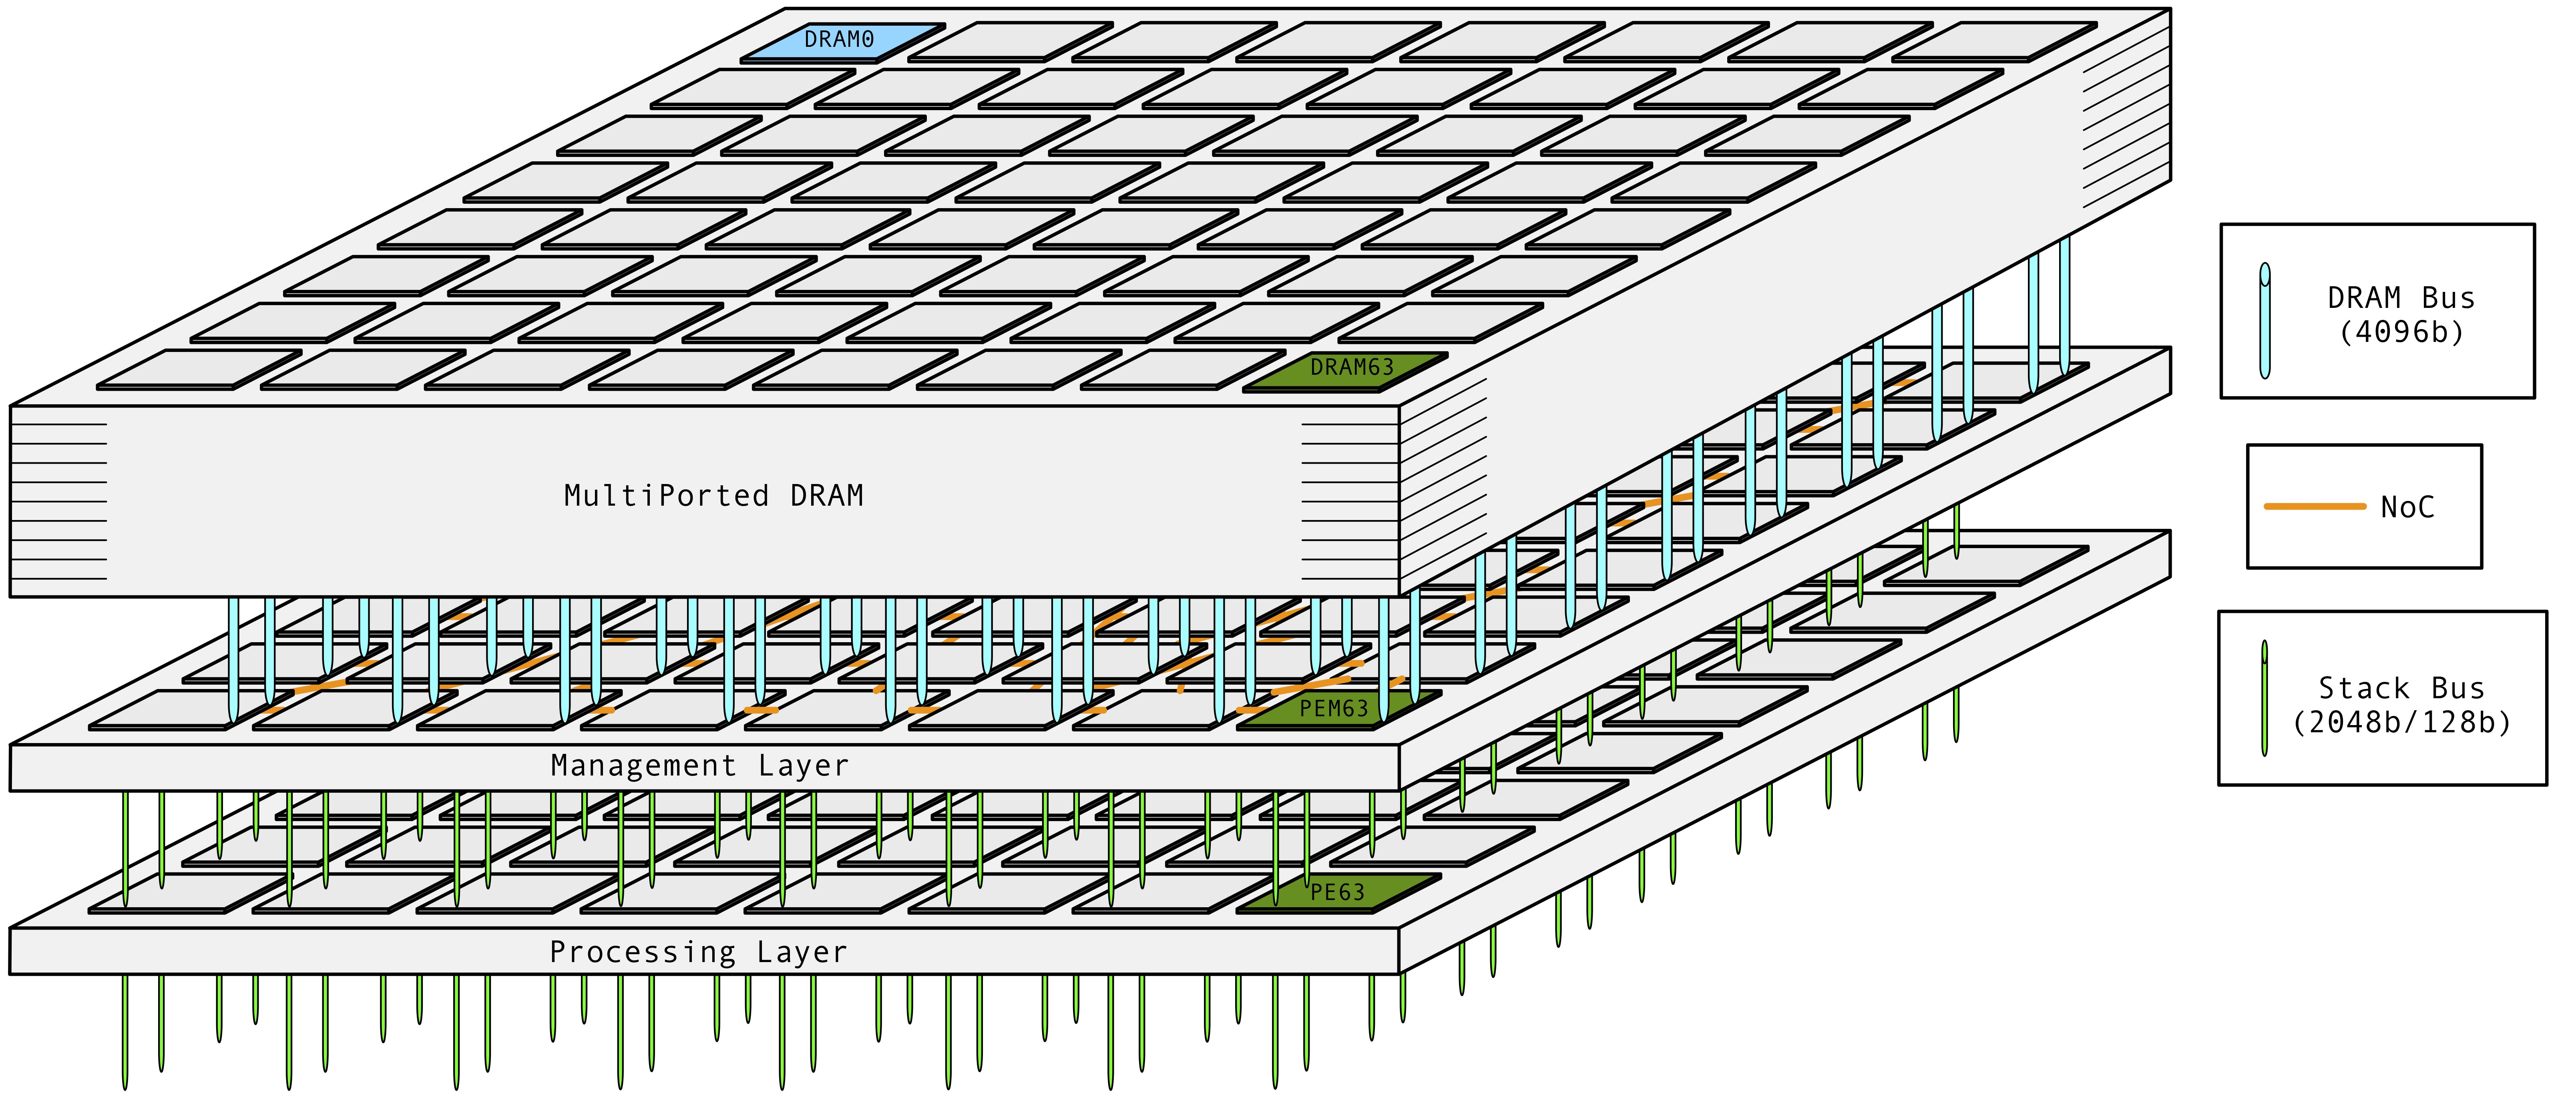
\includegraphics[width=1\textwidth]{SmallStackDiagram.jpg}
  \captionsetup{justification=centering, width=.8\linewidth}
  \caption{\ac{dram}, Manager and PE Layers}
  \label{fig:3DICStack}
\end{subfigure}%

\bigskip

\begin{subfigure}{.35\textwidth}
  \centering
  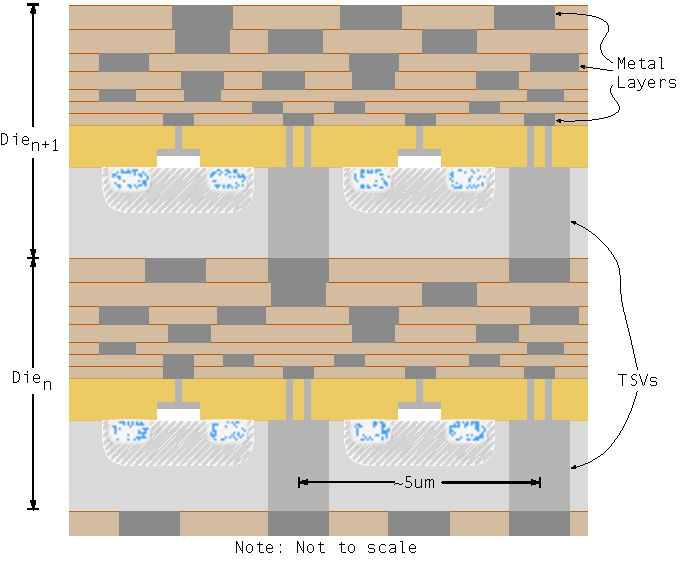
\includegraphics[width=1\textwidth]{TSVs.pdf}
  \captionsetup{justification=centering, width=1\linewidth}
  \caption{Example Stack profile with metal layers and TSVs \cite{itrs2015_interconn}}
  \label{fig:tsv}
\end{subfigure}
\captionsetup{justification=centering, width=.9\linewidth}
\caption{3DIC System Stack}
\label{fig:3DICStack}
\end{figure}

3D-\ac{dram} has recently become available in standards such as High Bandwidth Memory (HBM) and Hybrid Memory Cube (HMC) and proprietary devices such as the DiRAM4 available from Tezzaron. 
These technologies provide high capacity within a small footprint.

In the case of HBM and DiRAM4, the technology can be combined with additional custom layers to provide a system solution.

The question becomes, can a useful system coexist within the same 3D footprint?

This work targeted a baseline system with:
\begin{itemize}
  %\itemsep0em 
  \item single precision floating point for computations
  \item the Tezzaron DiRAM4 \ac{dram} \cite{tezzaron:diram4}
\iffalse
  \item target single precision floating point for computations
  \item use the Tezzaron DiRAM4 \ac{dram} for area estimates and memory controller design
\fi
\end{itemize}
The work includes customizing the interface to a 3D-\ac{dram}, researching data structures to describe storage of \ac{ann} parameters, designing a memory manager with micro-coded instructions and a processing engine (PE) layer.  
The targeted 3D-\ac{dram}, the Tezzaron DiRAM4 is a 3D-\ac{dram} employs multiple memory array layers in conjunction with a control and IO layer.
The memory is formed from 64 disjoint sub-memories each providing upwards of 1Gigabit with a total capacity of at least 64 gigabit.
The system is designed such that a sub-system, known as a sub-system column (SSC) operates on one of the 64 disjoint memories within the 3D-\ac{dram} (see Figure \ref{fig:diram4Layout}).

When the sub-system columns need to share data or neuron activations, the data is passed between SSCs using a mesh connected network-on-chip (NoC).

\bigskip
A control and data block diagram of the 3DIC stack showing the 64 sub-system columns can be seen in Figure \ref{fig:FlowDiagram}.
A block diagram of the sub-system column can be seen in Figure \ref{fig:DetailedFlowDiagram}. \iffalse and \ref{fig:DetailedBlockDiagram} respectively. \fi

\bigskip
An overview of the various blocks and interconnects are given below:

% ----------------------------------------------------------------------------------------------------
\subsection{3D-\ac{dram}}
The targeted 3D-\ac{dram}, the Tezzaron DiRAM4 is customized to provide a 2048-bit wide bus. A read to the memory using a burst of two cycles provides access to an entire page within a bank.
These customizations to support this very wide bus are discussed in \ref{sec:Suggested DRAM Customizations}.
The wide bus is connected to the manager using TSVs and the manager directs portions of the wide bus to each lane to the PE.
\begin{figure}[!t]
% the [] contains position info e.g. [!t] means here
\captionsetup{width=.9\linewidth}
\centerline{
\mbox{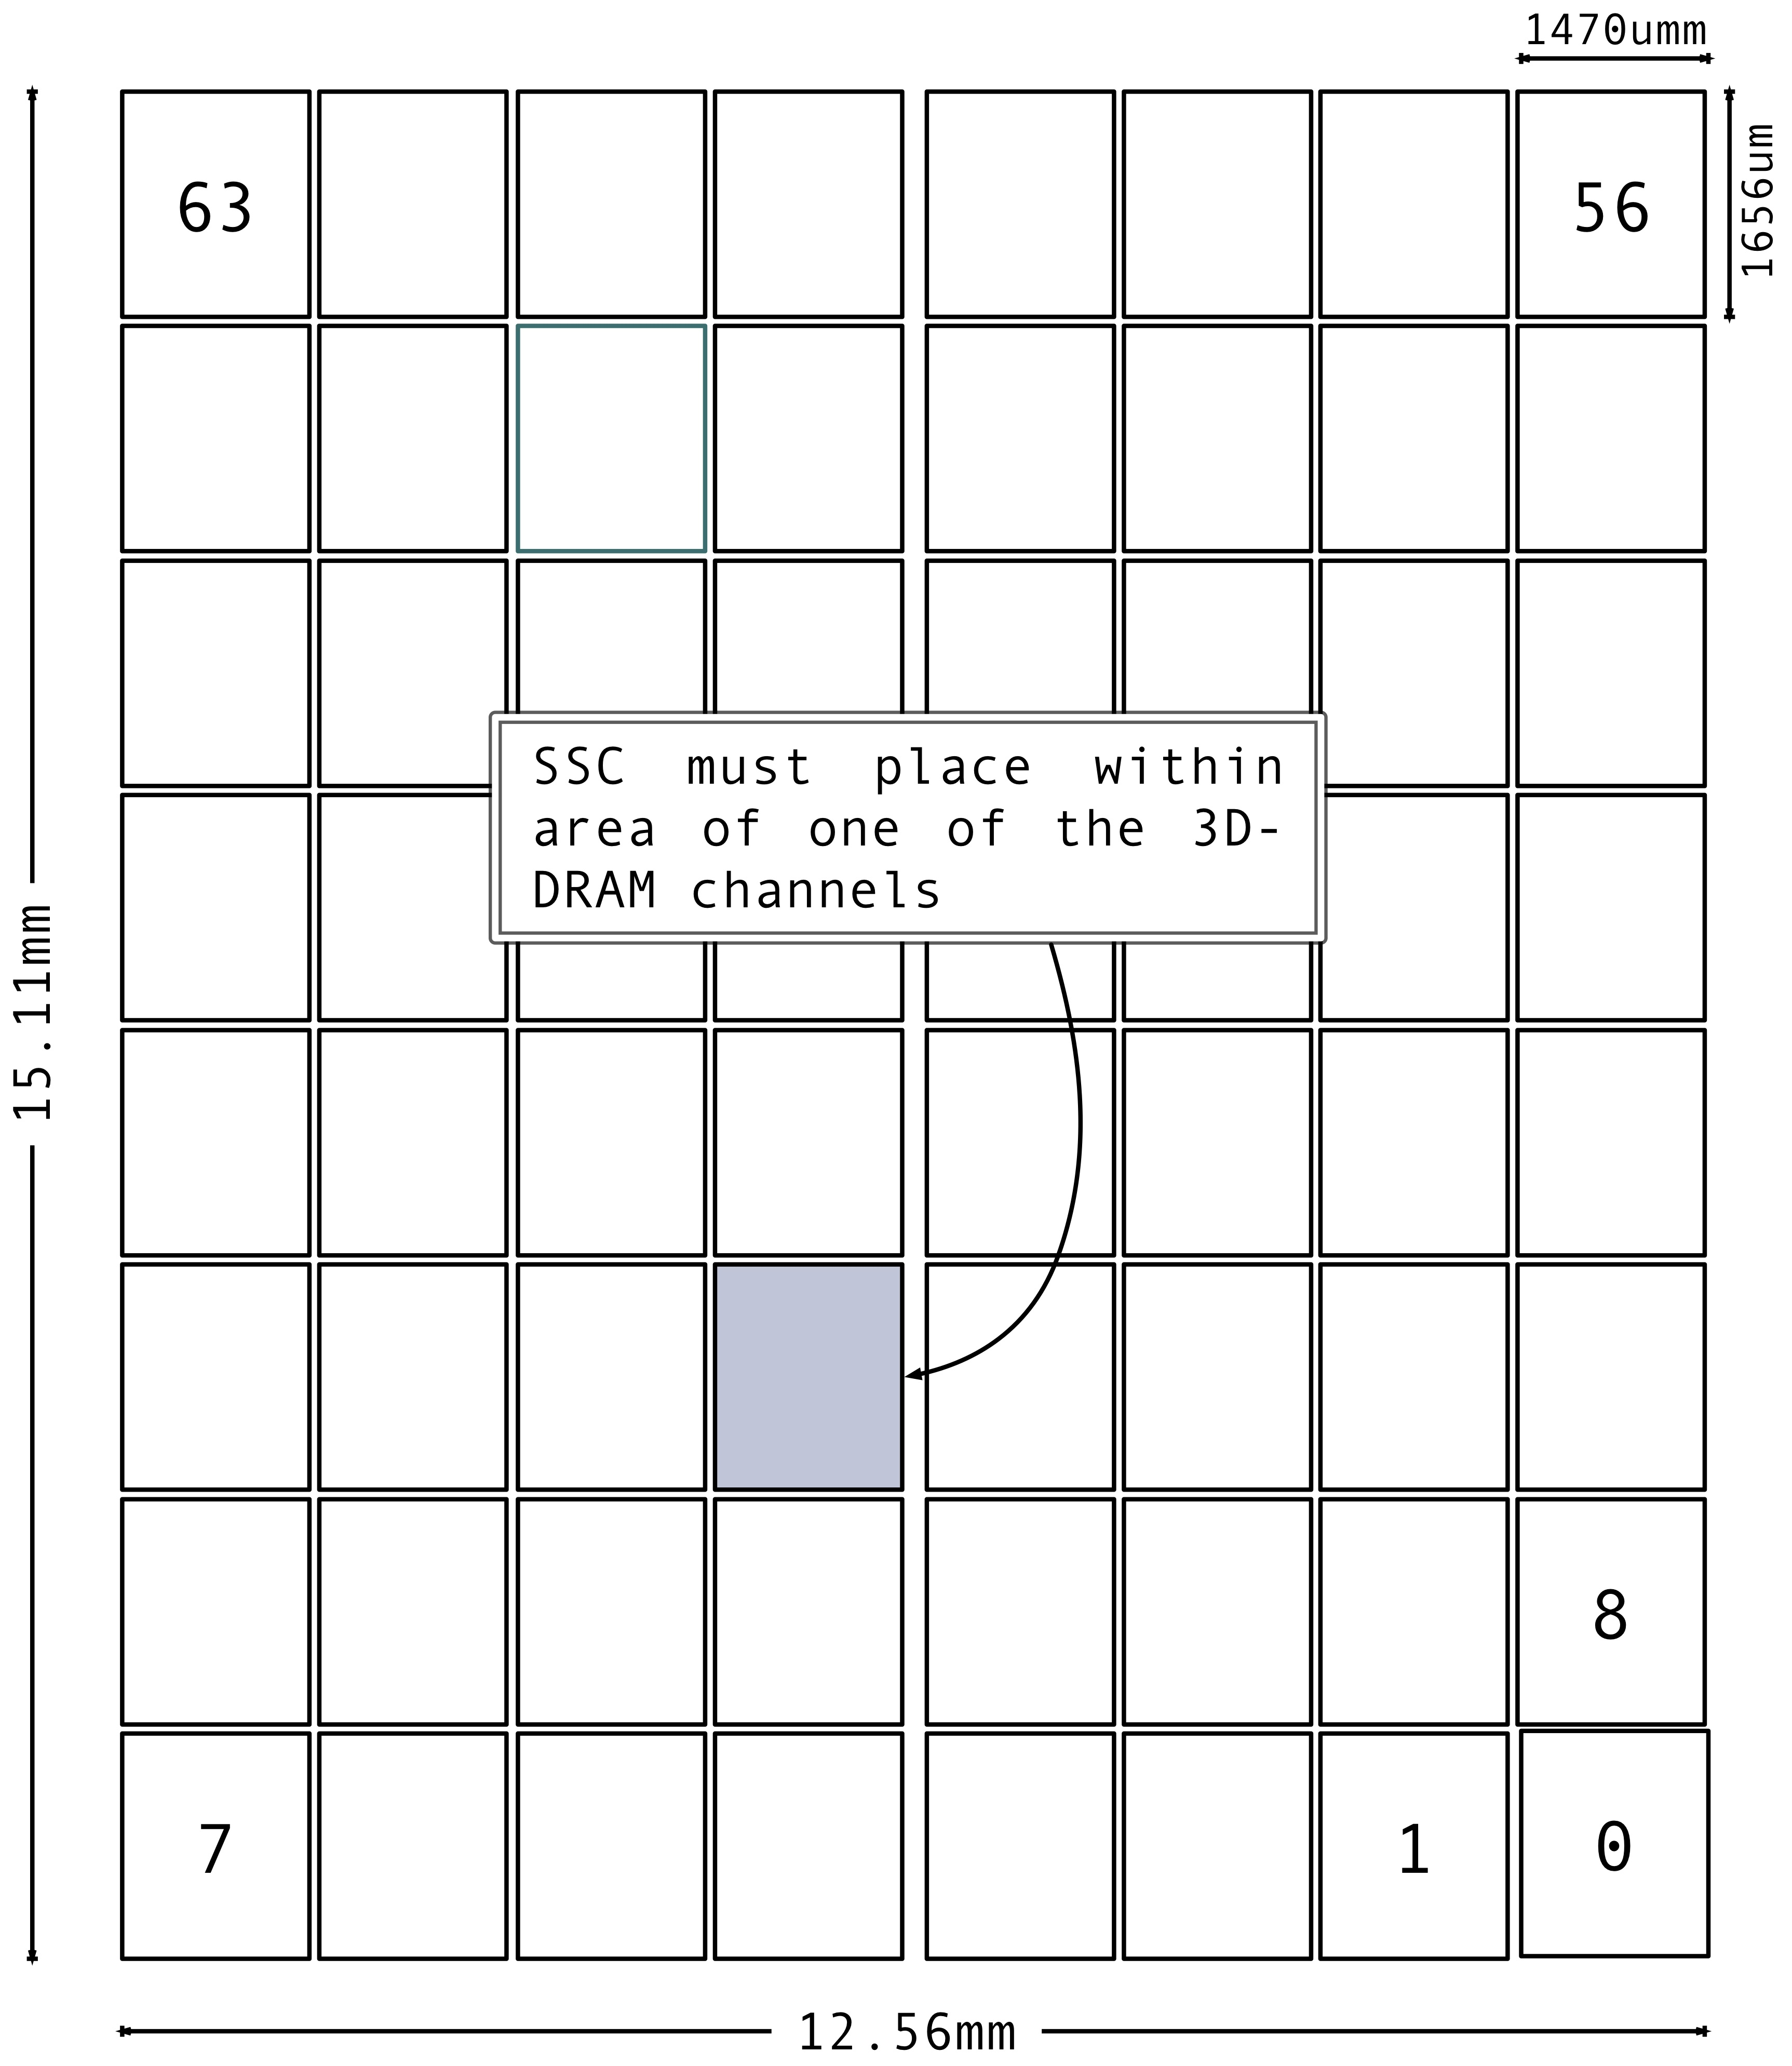
\includegraphics[width=2.5in]{DiRAM4Layout.jpg}}
}
\caption{DiRAM4 \ac{dram} Physical Interface Layout\cite{tezzaron:diram4}\cite{patti2014} showing area for SSC }
\label{fig:diram4Layout}
\end{figure}


% ----------------------------------------------------------------------------------------------------
\subsection{Manager Layer}
The Manager block is the main controller in the system. The operations required to process an \ac{ann} are formed from individual instructions which are decoded by the Manager. 
These instructions include descriptors to describe memory read operations, processing engine operations and memory write operations. The manager reads these system instructions from an instruction memory, decodes the instruction and configures the various blocks in the system.
The configuration includes:
\begin{itemize}

      \item initiate operand reads from \ac{dram}
      \item prepare the processing engine (PE) to operate on the operands
      \item prepare the result processing engine to take the resulting neuron activations from the PE and write those results back to the \ac{dram}
      \item replicate the resulting neuron activation's to neighbor managers for processing of other \ac{ann} layers

\end{itemize}

% ----------------------------------------------------------------------------------------------------
\subsection{Processing Layer}
\label{ssec:Processing Layer}
The PE is able to operate on data streamed directly from the \ac{dram} via the Manager layer. The PE is configured by the manager to perform operations on the operand data streamed from the manager. In the baseline system, the main operation is to perform multiply-accumulates on 32 execution lanes of two operands. These operands typically are the pre-synaptic neuron activation's and the connection weights. The PE also performs the activation function on the result of the MAC to generate the neuron activation value. These 32 activation values are sent back to the Manager layer.

% ----------------------------------------------------------------------------------------------------
\subsection{Layer Interconnect}
\label{ssec:Layer Interconnect}

The layers are connected using through-silicon-vias (TSVs) which provide high connection density, high bandwidth and low energy.
Figure \ref{fig:tsv} shows an example of two die connected using TSVs.
\iffalse
By ensuring the system stays within the 3D footprint ensures we can take advantage of the huge benefits provided by TSVs.
\fi

% ----------------------------------------------------------------------------------------------------
\subsection{Inter-Manager Communication}
\label{ssec:Inter-Manager Communication}

A Network-on-Chip (NoC) allows each management block to communicate with other managers.

\iffalse
This NoC has a forwarding table that can be reconfigured to provide more efficient routing for a given processing step.
\fi

During configuration and/or computations, data must be transported between managers. This inter-manager communication is provided by an NoC.
When computing an \ac{ann} across multiple processors, often neuron activation data must be shared. 
Each manager contains a NoC module and all the managers are connected in a mesh network.
\iffalse
The NoC architecture includes the ability to multicast where a NoC packet gets replicated as it traverses the mesh.
\fi
The NoC bandwidth was chosen to ensure the results can be multicast to any destination manager without an adverse affect on the pipelined instructions.
The NoC bus width is 64 data bits plus control signals running at the system clock rate. Future testing may require additional NoC bandwidth.

\iffalse
The SSC includes the \ac{dram} port, the manager and the PE. 
\fi

\begin{figure}[!t]
% the [] contains position info e.g. [!t] means here
\centering
\captionsetup{justification=centering}
\centerline{
\mbox{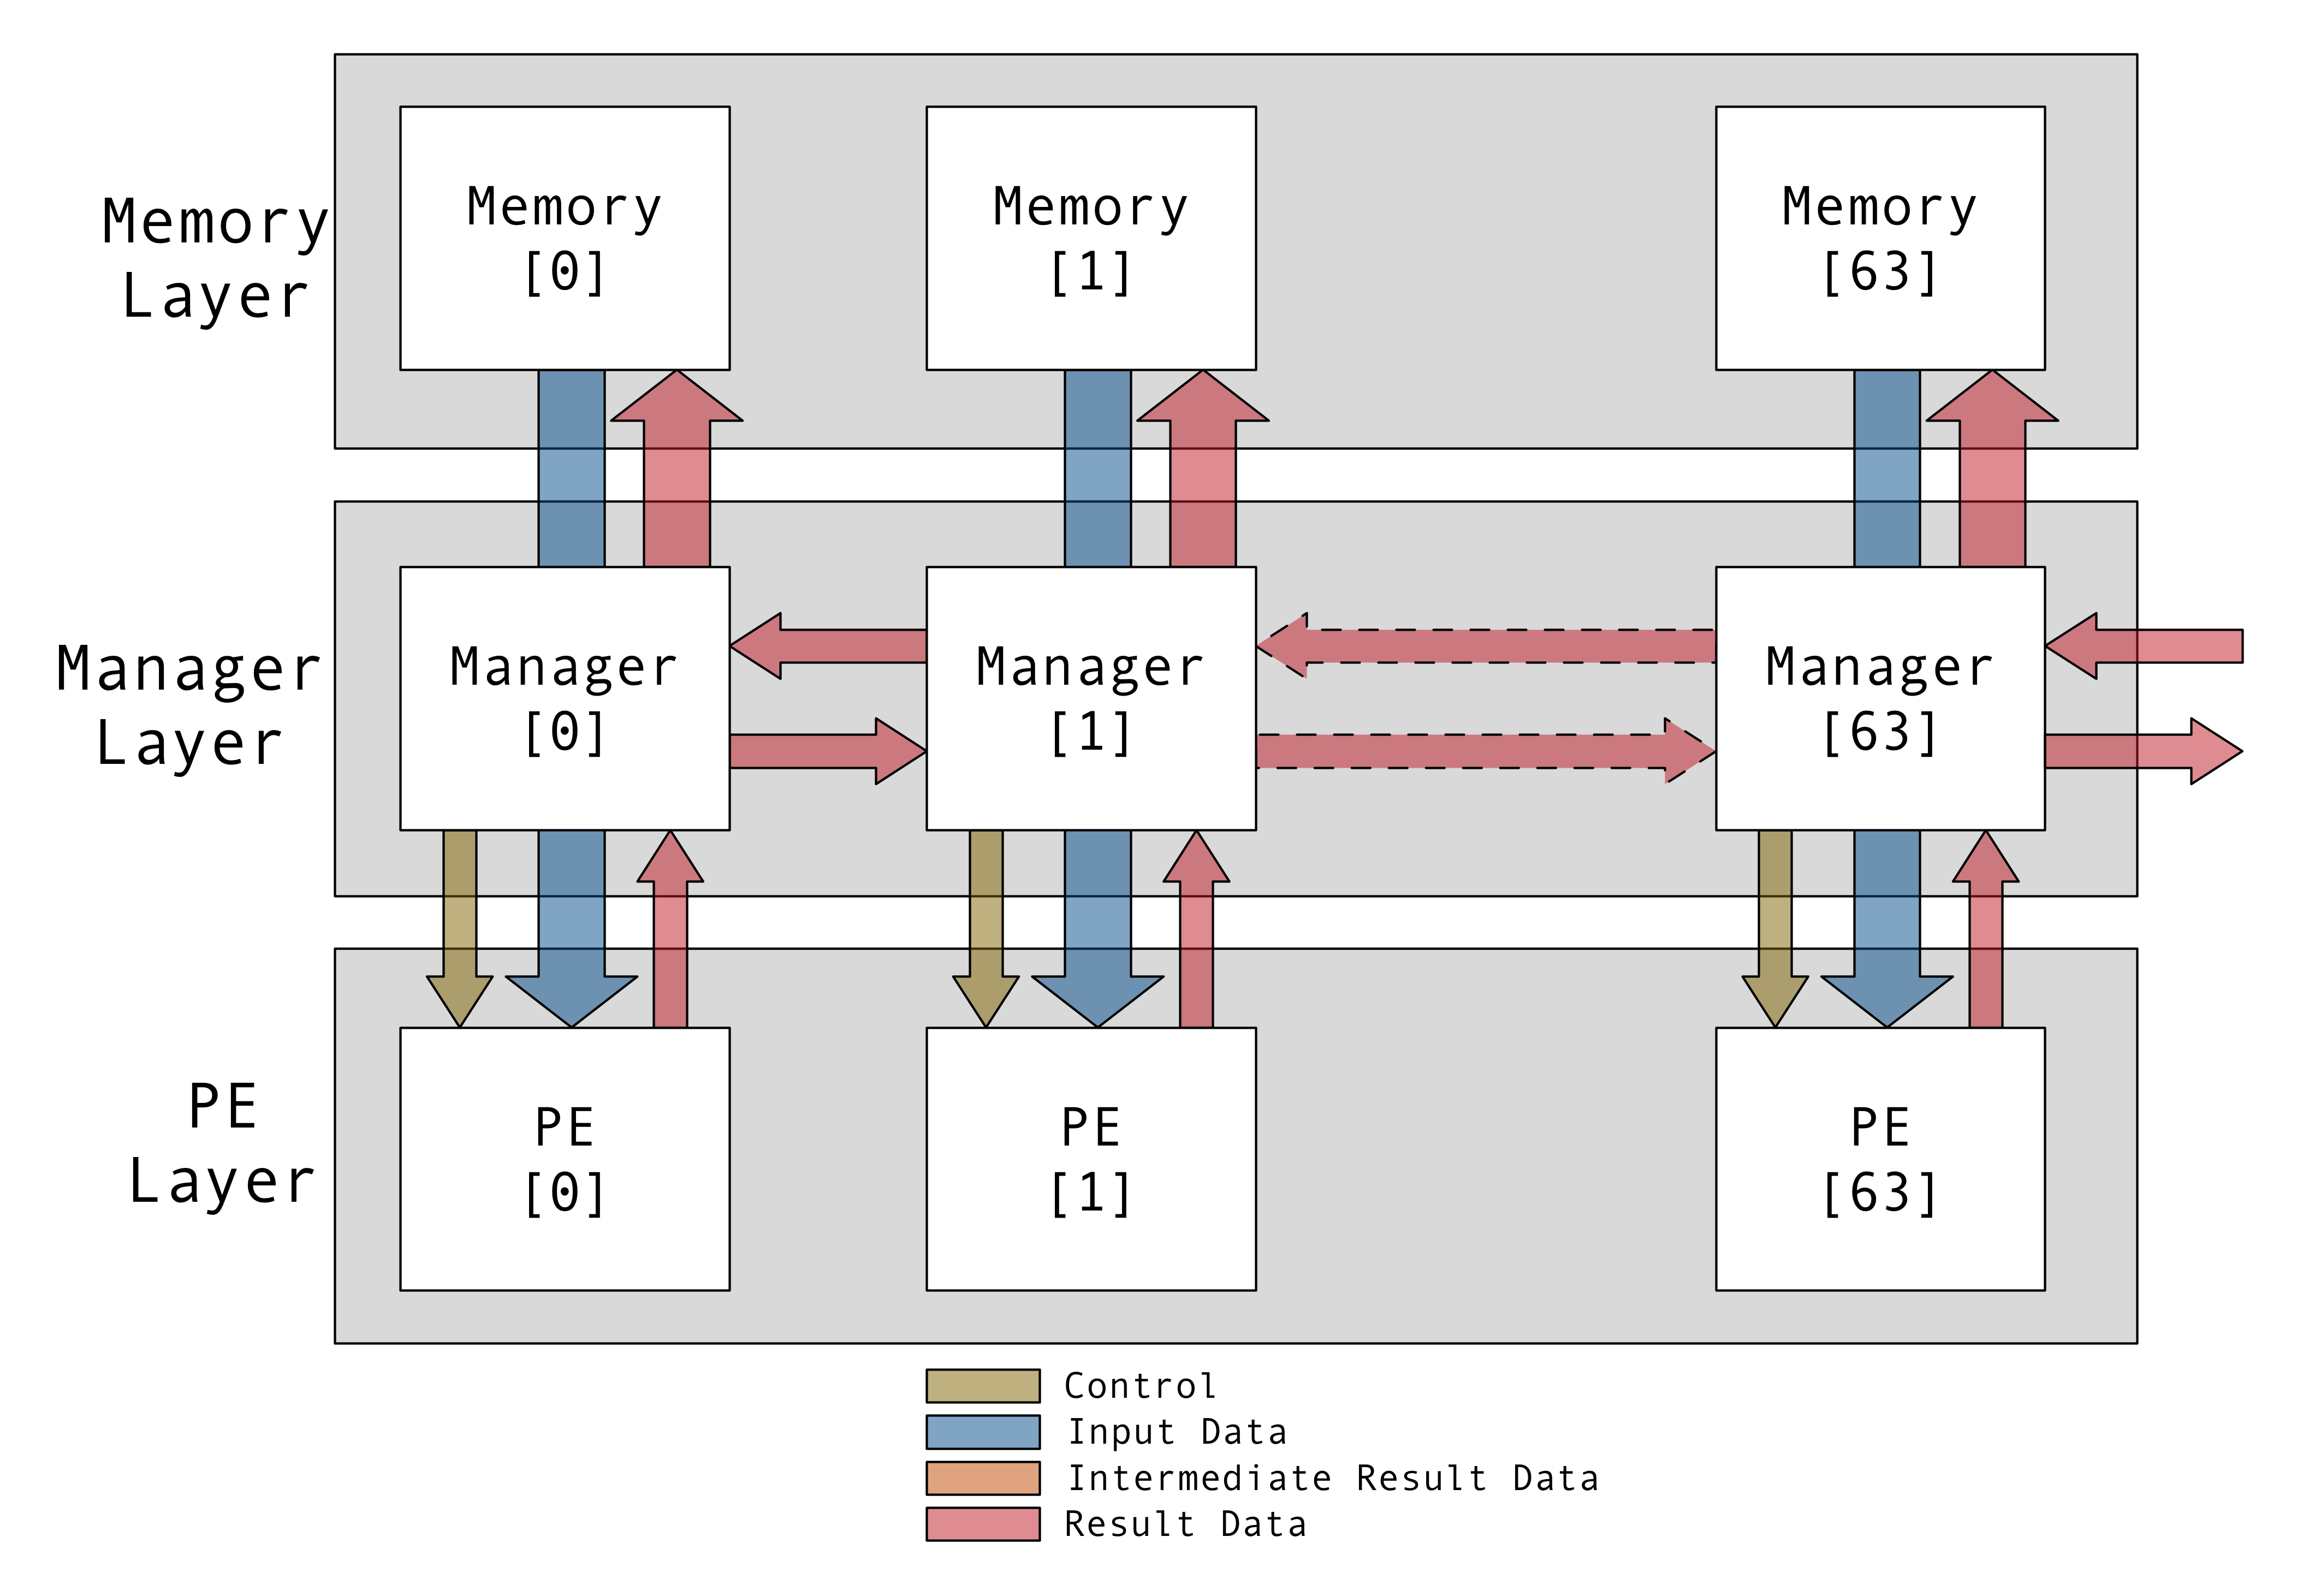
\includegraphics[width=3.0in]{FlowDiagram.jpg}}
}
\caption{System Diagram}
\label{fig:FlowDiagram}
\end{figure}


% >>>>>>>>>>>>>>>>>>>>>>>>>>>>>>>>>>>>>>>>>>>>>>>>>>>>>>>>>>>>>>>>>>>>>>>>>>>>> System Operations <<<<<<<<<>>>>>>>>>>>>>>>>>>>>>>>>>>>>>>>>>>>>>>>>>>>>>>>>>><<<<<<<<<<<<<
\section{System Operations}
\label{sec:System Operations}
In the context of this system and \ac{an} state calculation, the basic operations to determine the state of a neuron is to:

\begin{itemize}
    \item Inform the Manager and PE which operations are to be performed
    \item Instruct the manager to access the states of the pre-synaptic neurons
    \item Instruct the manager to access the weights of the connections from the pre-synaptic \acp{an}
    \item Provide the pre-synaptic neuron weights and states to the processing engine execution lanes
    \item Instruct the manager where to store the resulting \ac{an} state back to memory
\end{itemize}

This work has researched an instruction architecture to describe the above operations. 
These instructions are decoded by the manager. 

In the baseline system, the manager is not responsible for performing specific algorithm operations but is responsible for coordinating the various data flows and configuration of the modules that make up the system.

The managers primary responsibility is:

\begin{outline}
    \1 Instruction decode
    \1 Internal Configuration messages
    \1 Operand read
    \1 Result write
\end{outline}

In the baseline system, the PE is responsible for the main algorithm operations.

The PE has three major blocks:

\begin{outline}
  %\setlength{\baselineskip}{10pt}
  %\setlength{\itemsep}{6pt}
    \1 \ac{stop} 
      \2 Processes data from the manager on-the-fly without storing in local \ac{sram}
    \1 \ac{simd}
      \2 Processes the data from the \ac{stop} function
        \3 Neuron activation function such as ReLu
        \3 Perform non vector operations such as softmax conversion using local \ac{simd} functions, such as $e^x$ and divide
      \2 Sends the result back to the manager
    \1 DMA/local memory controller
      \2 Transfer configuration data to PE conroller or to store \ac{stop} results to a small local \ac{sram} which can be used for access by \ac{simd} or by the \ac{stop} function
\end{outline}
% ----------------------------------------------------------------------------------------------------
% ----------------------------------------------------------------------------------------------------
\subsection{Manager Operations}
\label{sec:Manager Operations}

% ----------------------------------------------------------------------------------------------------
\subsubsection{Instructions}
\label{ssec:Instructions}
The instructions include information to control the following operations.

\begin{outline}
  %\setlength{\baselineskip}{10pt}
  %\setlength{\itemsep}{6pt}
  %\setlength{\baselineskip}{10pt}
  %\setlength\itemsep{0pt}
  %\setlength{\partopsep}{0pt}
  %\setlength{\parskip}{0pt}
  %\setlength{\parsep}{0pt}
  %\setlength{\topsep}{0pt}
  %\setlength{\itemsep}{3pt}
  %\setlength{\itemindent}{\leftmargin}
  %\setlength{\leftmargin}{0pt}
        \1 To the Manager
            \2 \ac{roi} Storage descriptor
            \2 Parameter/Weight Storage Descriptor
                \3 Broadcast or Vectored
            \2 Result write storage descriptor
                \3 include descriptors for all destination managers
        \1 To the PE
            \2 \ac{stop} operation
            \2 \ac{simd} operation
            \2 Number of active lanes
            \2 Operand Vector length
\end{outline}


Instructions contain sub-instructions called descriptors. 
These descriptors contain the information to control the various operations associated with the processing of a group of \acp{an}.
The group size is related to the number of execution lanes which for the baseline system is 32. A group can be anywhere from 1-32. It should be said that unless the group size consistently approaches 32 the system performance will be poor.

An instruction will typically have four descriptors:

\begin{outline}
\renewcommand{\outlinei}{enumerate}
    \1 Operation
    \1 Memory read for operand stream 0
    \1 Memory read for operand stream 1
    \1 Result Write
\end{outline}

The instruction is an n-tuple where the tuple elements are descriptors and the number of elements can vary based on the operation being performed. In Figure \ref{fig:instructionTuple} is shown the format of a 4-tuple instruction which is used to perform an activation calculation for a group of neurons.

\begin{figure}[!t]
\centerline{
\mbox{
\includegraphics[width=2.75in]{instruction4Tuple.jpg}}
}
\caption{Instruction 4-tuple}
\label{fig:instructionTuple}
\end{figure}

\iffalse
Within a descriptor there are fields to describe the various options such as storage descriptor pointer, number of operands etc..
\fi

The fields within the descriptor are n-tuples where the first tuple element describes the descriptors operation followed by an m-tuple whose elements contain the options required for the operation.

These option elements are a two-tuple with option and associated value.
The format of a 5-tuple descriptor can be seen in Figure \ref{fig:descriptorTuple} .

\begin{figure}[!t]
\centerline{
\mbox{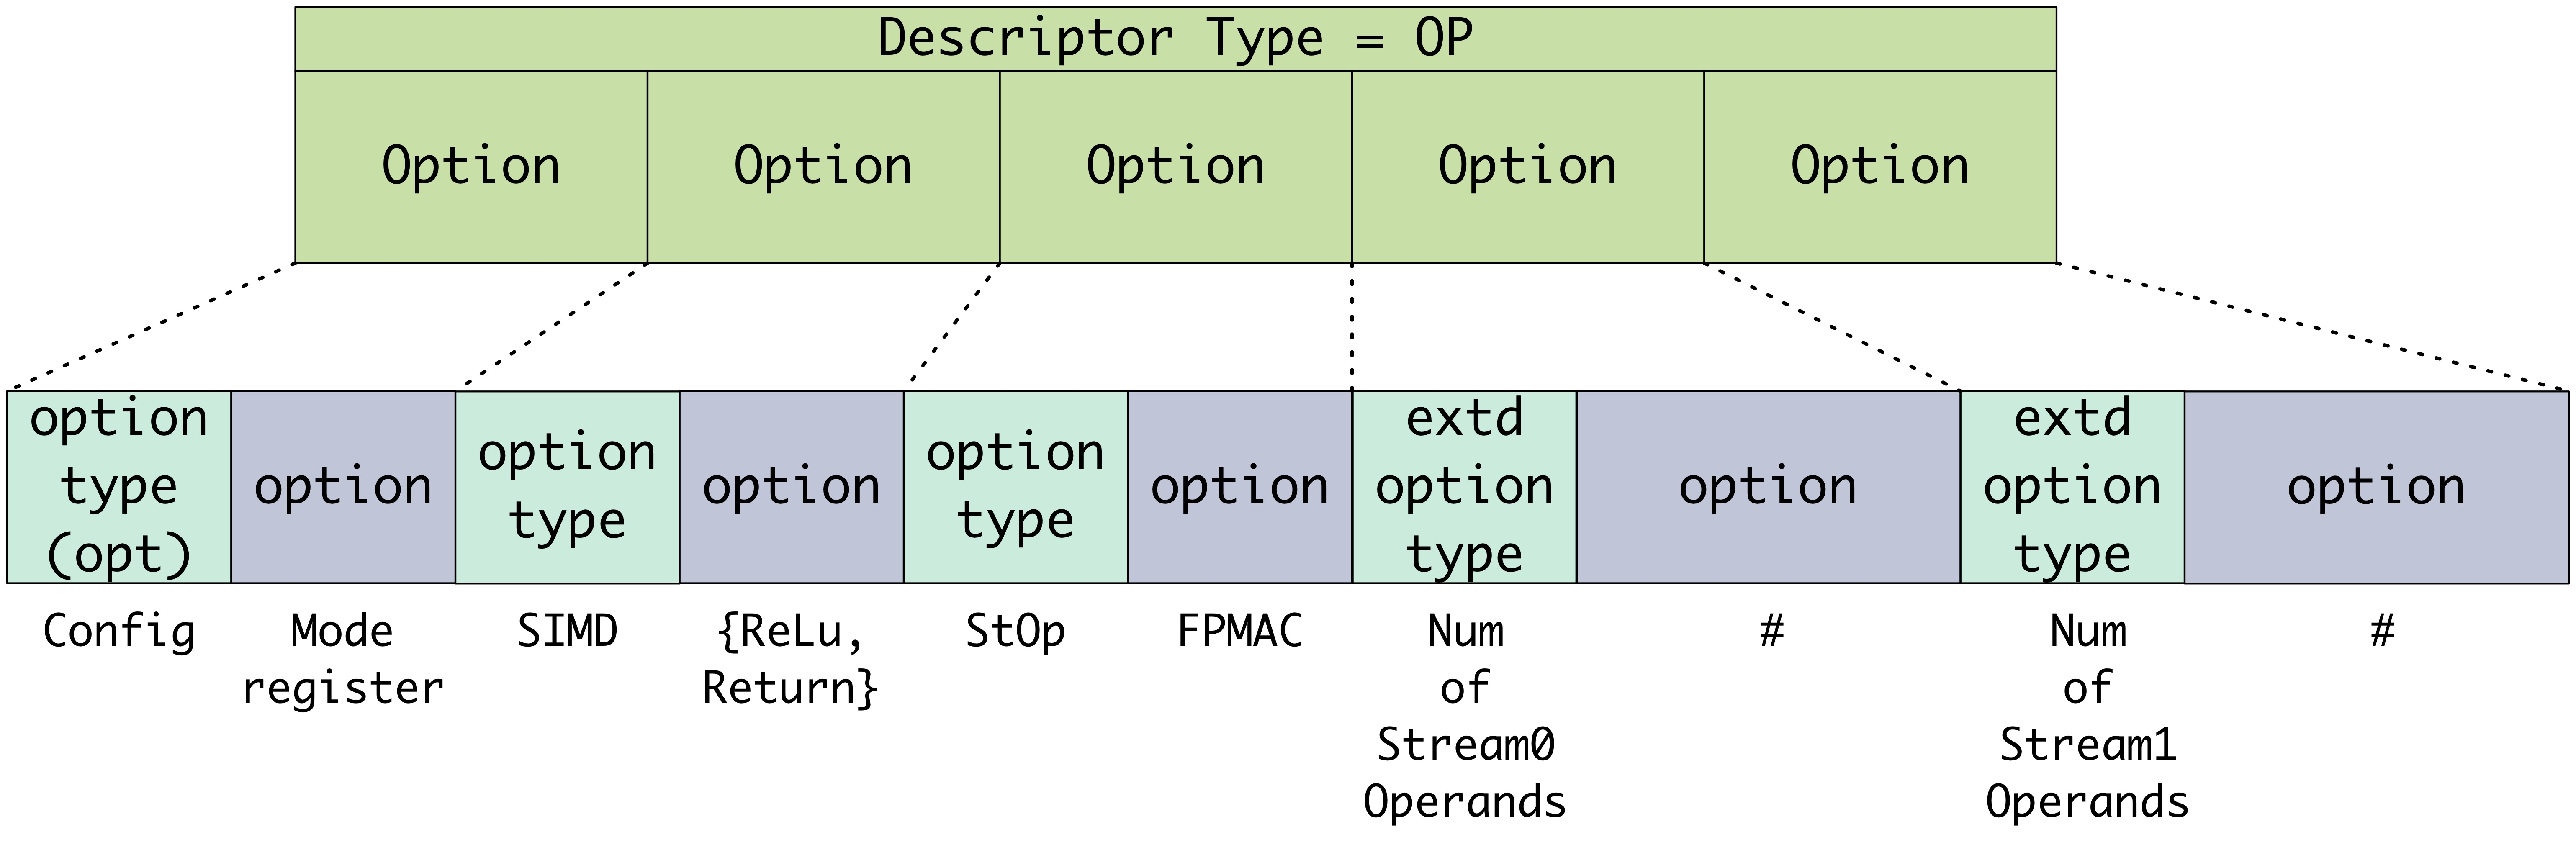
\includegraphics[width=2.75in]{descriptorTuple.jpg}}
}
\caption{Descriptor 5-tuple}
\label{fig:descriptorTuple}
\end{figure}

%%%% Feedback from Paul
%%%%  % ----------------------------------------------------------------------------------------------------
%%%%  \subsubsection{Accessing of Pre-synaptic \ac{an} states and connection weights}
%%%%  \label{ssec:AccessingANStates}
%%%%  
%%%%  As was discussed previously, the \ac{ann} input and configuration is stored in main \ac{dram} memory. A part of the research is determining how to store the \ac{ann} input and parameters in such a way to effectively make use of main \ac{dram} bandwidth. To provide parameters for the up to 32 execution lanes within the PE, the \ac{an} parameters are stored in consecutive address locations. A single read to the \ac{dram} accesses 128 words. This provides four weights for each of the 32 \acp{an} being processed. 
%%%%  These weights are sent to each lane of the PE over four cycles. 
%%%%  By taking advantage of the multiple \ac{dram} banks along with pre-fetching and buffering, this system is able to achieve relatively high efficiency of the available maximum bandwidth.
%%%%  
%%%%  Although \ac{an} parameters (weights) are stored in contiguous memory locations, providing the input state to a particular \ac{an} presents us with an interesting problem.
%%%%  
%%%%  Most often \acp{dnn}s are represented by layers of \acp{an} whose pre-synaptic neurons are from the previous layer. These previous layers represent the input to a given layer. The first layers input is the actual input to the \ac{ann}.
%%%%  
%%%%  The input can be represented in the form of a 2-D array of \ac{an} states. For the sake of generality, the input array elements are considered as \ac{an} states.
%%%%  
%%%%  Any given \ac{an} operates on a region of interest (ROI) within the layers input array.
%%%%  
%%%%  
%%%%  \begin{figure}[!t]
%%%%  \centerline{
%%%%  \mbox{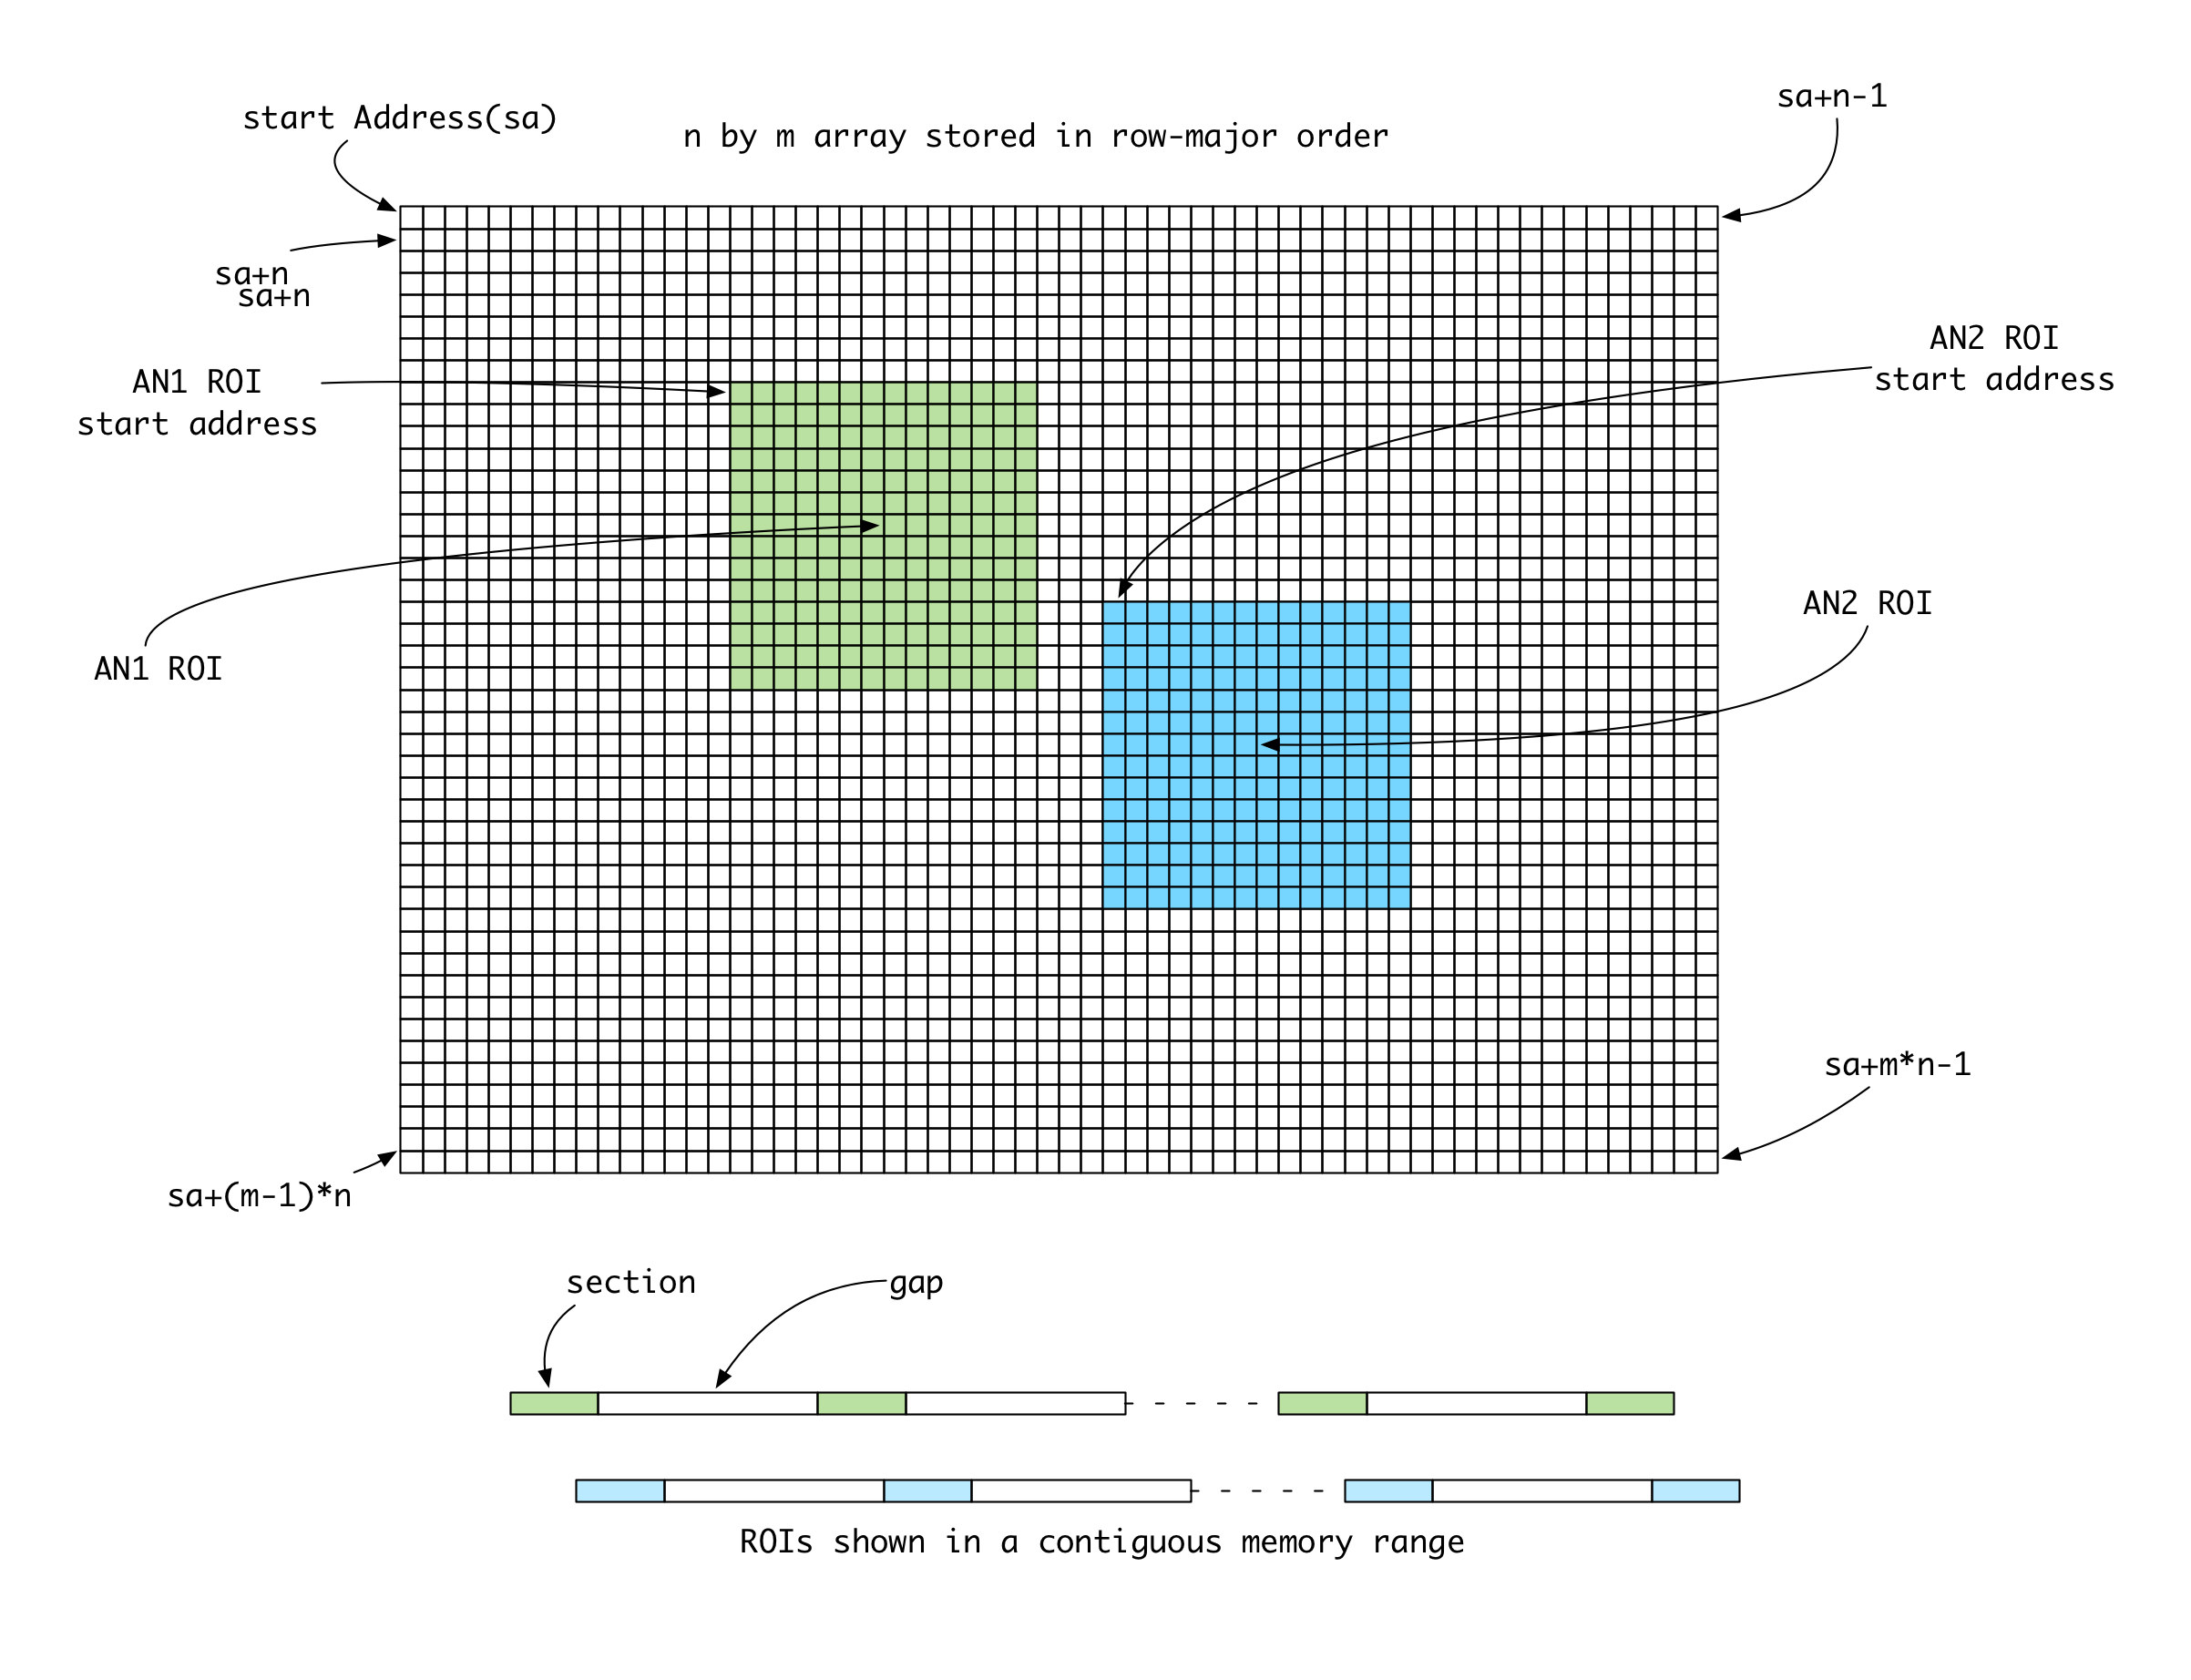
\includegraphics[width=2.75in]{roiStorage.jpg}}
%%%%  }
%%%%  \caption{ROI Storage}
%%%%  \label{fig:roiStorage}
%%%%  \end{figure}
%%%%  
%%%%  The various connection weights are stored in multiple contiguous sections. However, its not possible to arrange the input in such a way that each \acp{an} ROI can be stored in contiguous memory locations. 
%%%%  An input to a \ac{ann} layer in the form of a 2-D array along with the ROI of two \acp{an} is shown in Figure \ref{fig:roiStorage}. 
%%%%  Assuming the input array is stored in row-major order, an ROI is drawn from disjoint sections of memory. 
%%%%  These disjoint sections contain a number of \ac{an} states and the sections are separated by a gap of a number of memory addresses. When the parameters are accessed the memory controller within the manager must be informed of the start address and the lengths of the sections and gaps. 
%%%%  \iffalse
%%%%  Now this looks problematic, and it is, but in practice groups of \acp{an} share a common ROI. So once we solve the problem of efficiently reading an ROI from the \ac{dram}, that ROI can be shared across a group of \acp{an}
%%%%  \fi
%%%%  
%%%%  This work proposes a data structure to describe these ROI storage locations.  
%%%%  The ROI is read efficiently by taking advantage of the \ac{dram}s banks and pages.
%%%%  
%%%%  Although disparate groups of \acp{an} may have a different start addresses for their ROI, a commonality is observed in the ROI section lengths and gaps. So for each \ac{an} group, the groups ROI starting address is stored along with a pointer to a common set of section length/gaps. This structure is termed a storage descriptor.
%%%%  
%%%%  This storage descriptor contains the start address of the ROI and a pointer to a section/gap descriptor. 
%%%%  \iffalse
%%%%  Many storage descriptors point to a common section/gap descriptor. This avoids having to have a unique section/gap descriptors for each \ac{an} group.
%%%%  \fi
%%%%  
%%%%  Figure \ref{fig:storageDescriptor} shows the structure of the storage descriptor. The SOD, MOD and EOD are used to delineate each descriptor in memory and stand for start-of-descriptor, middle-of-descriptor and end-of-descriptor.
%%%%  To limit the amount of storage required, a repeat operation can also be used to use a pair of section/gap fields multiple times.
%%%%  
%%%%  \begin{figure}[!t]
%%%%  \centerline{
%%%%  \mbox{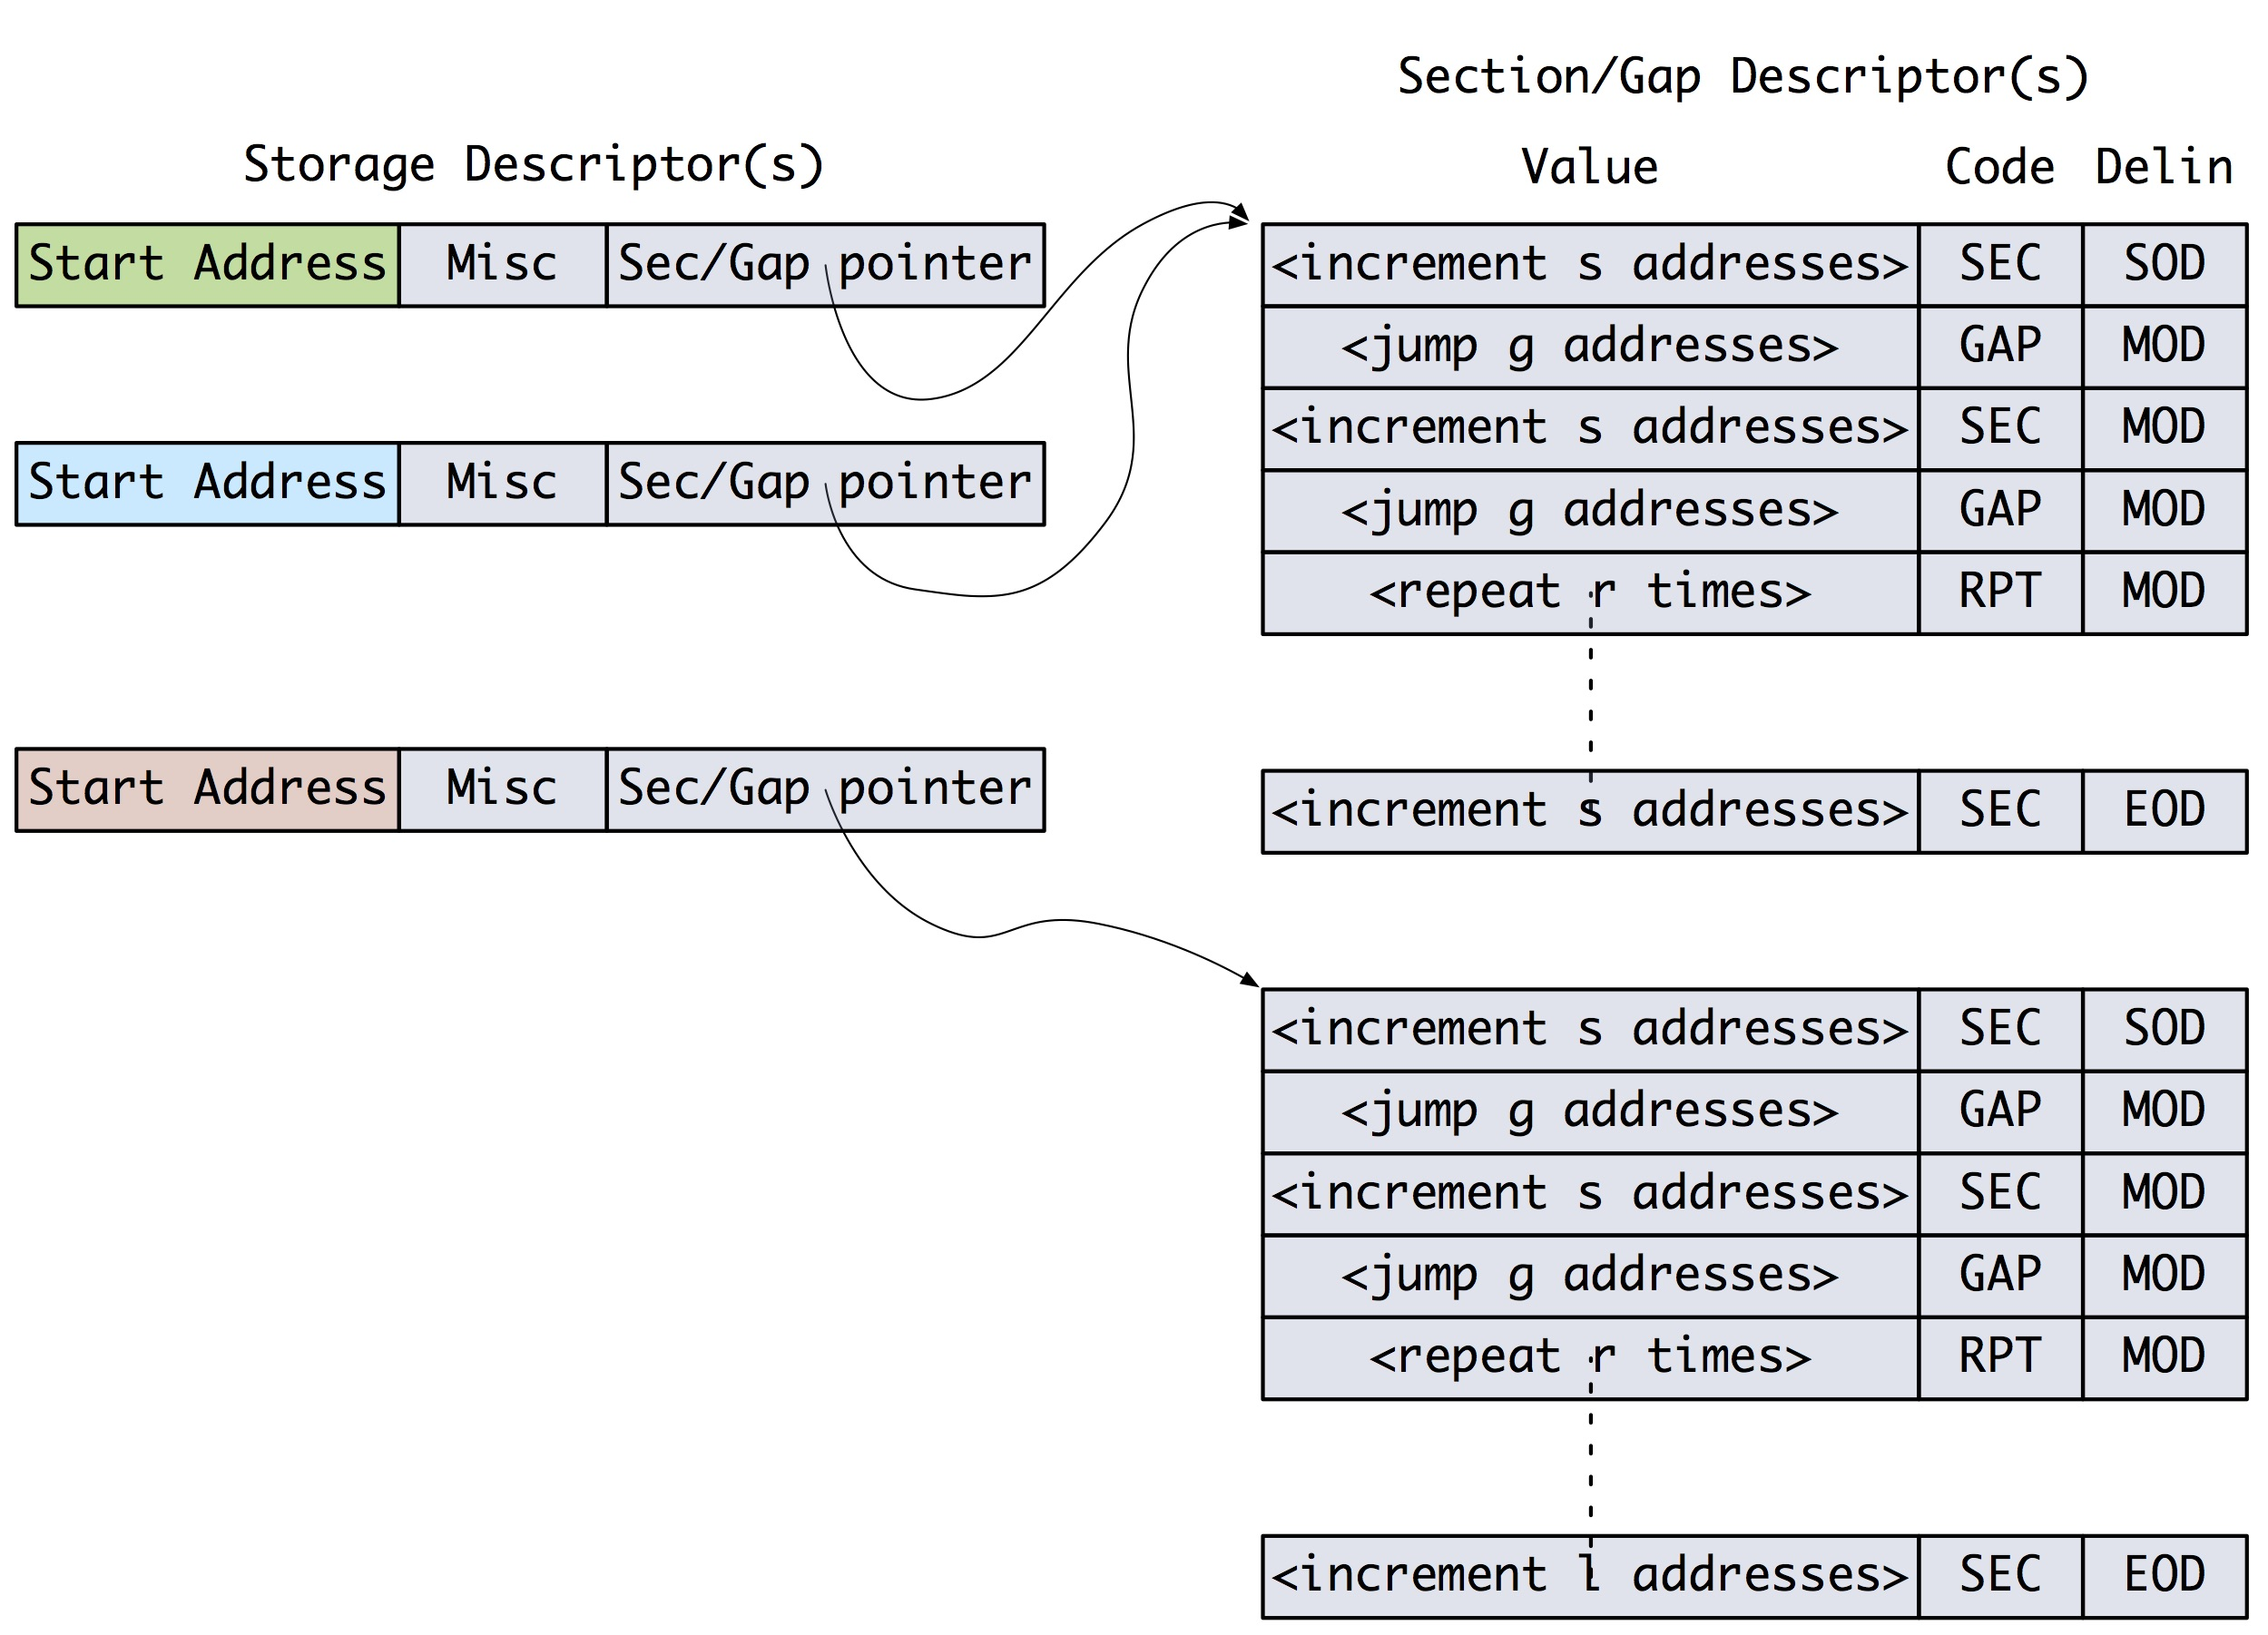
\includegraphics[width=2.75in]{storageDesc.jpg}}
%%%%  }
%%%%  \caption{Storage Descriptor}
%%%%  \label{fig:storageDescriptor}
%%%%  \end{figure}
%%%%  
%%%%  

% ----------------------------------------------------------------------------------------------------
\subsubsection{Write Back to Memory}
\label{ssec:writingANStates}

When the PE has processed the group of \acp{an}, the new \ac{an} states are sent back to the manager for storing in the \ac{dram}. 
\iffalse
The manager will store these back to \ac{dram} most likely in the array format as described earlier.
For any given operation, the system is writing far less than is being read. 
\fi

\iffalse
For example, the ROI and parameters are usually vectors that will typically exceed 100 elements and in many cases much higher. When an operation is complete, in almost all cases one word per lane is writen back to main memory. 
\fi

\iffalse
Now that sounds like writing back has a very small impact on performance but with \ac{dram}s that's not always true.
\fi

\iffalse
When the system writes the result of an operation back to memory, it is typically writing a small portion of a \ac{dram} page and the nature of the \ac{dram} protocol means this is a very inefficient use of \ac{dram} bandwidth. 
So although the amount of data written is small the performance impact c\ac{ann}ot be ignored.
\fi

In many cases the \ac{an} activations from a particular PE have to be replicated not only to the local manager but also to other managers. This is handled with the network-on-chip (NoC).
\iffalse
The result storage directives are communicated by using the same storage descriptor mechanism. When the result has to be replicated to other managers, the storage descriptors are sent, along with the data to all destination managers.
\else
When the result has to be replicated to other managers, the data is sent, along with storage information over the NoC to all destination managers.
\fi

% ----------------------------------------------------------------------------------------------------
% ----------------------------------------------------------------------------------------------------
\subsection{PE Operations}
\label{sec:PE Operations}

% ----------------------------------------------------------------------------------------------------
\subsubsection{\acf{stop}}
\label{ssec:streamingOps}
The operations performed by the \ac{stop} are primarily multiple-accumulate with a transfer to the \ac{simd} or to local memory.
\iffalse
Even though the baseline system focuses on the \ac{an} multiply-accumulate followed by a ReLu activation function, the system has built in flexibility into the \ac{stop} function to allow other functions to be added
\fi

In most cases, the \ac{stop} module will operate on the \ac{an} state and weights provided by the manager and provide the result to the \ac{simd}.
% ----------------------------------------------------------------------------------------------------
\subsubsection{SIMD}
\label{ssec:SIMD}

The \ac{simd} is a 32-lane processor with some builtin special functions including $e^x$ and divide to allow on-the-fly operations. 

The \ac{simd} will take the result provided by the \ac{stop} and perform additonal operations such as neuron activation, pooling or softMax. The result will then be transmitted back to the manager.
\iffalse
In some cases, the manager uses the result from a previous instruction on a following instruction, an example being a softMax operation.
\fi

% ----------------------------------------------------------------------------------------------------
\subsubsection{Configuration}
\label{ssec:peConfiguration}

To configure the PE operations, the manager extracts two pointers from the instruction and sends them in a configuration packet to the PE. These pointers index into a small local memory which provides a program counter (PC) to the function to be performed by the \ac{simd} and a configuration entry for the operation to be performed by the stOp.
 
\iffalse
The PE is able to perform its operation concurrently on 32-lanes. 
In cases when less than 32-lanes will be employed, the configuration packet also provides the number of lanes being processed.
In addition, the length of the vector of operands is contained in the configuration packet.
\fi

\bigskip
A detailed block diagram of the sub-system column (SSC) can be seen in Figure \ref{fig:DetailedFlowDiagram}.

% >>>>>>>>>>>>>>>>>>>>>>>>>>>>>>>>>>>>>>>>>>>>>>>>>>>>>>>>>>>>>>>>>>>>>>>>>>>>> \ac{dram} Customizable <<<<<<<<<>>>>>>>>>>>>>>>>>>>>>>>>>>>>>>>>>>>>>>>>>>>>>>>>>><<<<<<<<<<<<<
\section{Suggested DRAM Customizations}
\label{sec:Suggested DRAM Customizations}

Accessing a "typical" \ac{dram} involves opening a page in a bank, reading or writing a portion of the contents of the page then closing the page.

Typically a bank may contain of the order of a few thousand pages and a page may contain of the order of a few thousand bits.

Once the page is open, the user accesses a portion of the requested page over a bus. With PCB based \ac{dram}s the bus might vary from four to 16 bits wide, but with 3D \ac{dram}s, such as HBM the bus might be up to 128 bits wide.

\iffalse
Figure \ref{fig:\ac{dram}BlockDiagram} shows a block diagram of a typical \ac{dram}.

\begin{figure}[!t]
% the [] contains position info e.g. [!t] means here
\centering
\captionsetup{justification=centering}
\centerline{
\mbox{\includegraphics[width=2.75in]{\ac{dram}BlockDiagram.jpg}}
}
\center\caption{Typical \ac{dram} Block Diagram}
\label{fig:\ac{dram}BlockDiagram}
\end{figure}

\fi

\subsection{Expose more of the Page}
\label{sec:exposeMorePage}

This work achieves the increase in bandwidth by proposing that the \ac{dram} expose more of its currently open page.

Without the limitations of having to transfer data beyond the chip stack, this work suggests exposing a larger portion of the page over a 2048-bit wide bus. By staying within the 3D footprint, this bus can be implemented using fine pitch TSVs.
(see Figure \ref{fig:DRAMBusChange}).

\begin{figure}[!t]
% the [] contains position info e.g. [!t] means here
\centering
\captionsetup{justification=centering}
\captionsetup{width=.9\linewidth}
\centerline{
\mbox{\includegraphics[width=2.75in]{dramBusChange.jpg}}
}
\center\caption{Exposing more of the \ac{dram} page}
\label{fig:DRAMBusChange}
\end{figure}

\subsection{DRAM Write Mask}
\label{sec:DRAMWriteMask}
For every group of \acp{an} processed, the state of the group of \acp{an} is written back to memory.
Typically this would require a read/modify/write of a \ac{dram} cacheline. In the case writing back 32 \ac{an} states into a 4096 bit cacheline means the read/modify/write is inefficient.
To minimize the inefficiency, a customization to the \ac{dram} is the addition of a write data mask to the \ac{dram} write path eliminating the additional read.


% #######################################################################################################################################
%
%            IFFALSE
%
% #######################################################################################################################################
\iftrue

\begin{figure}[!t]
% the [] contains position info e.g. [!t] means here
\centering
\captionsetup{justification=centering}
\captionsetup{width=.9\linewidth}
\centerline{
\mbox{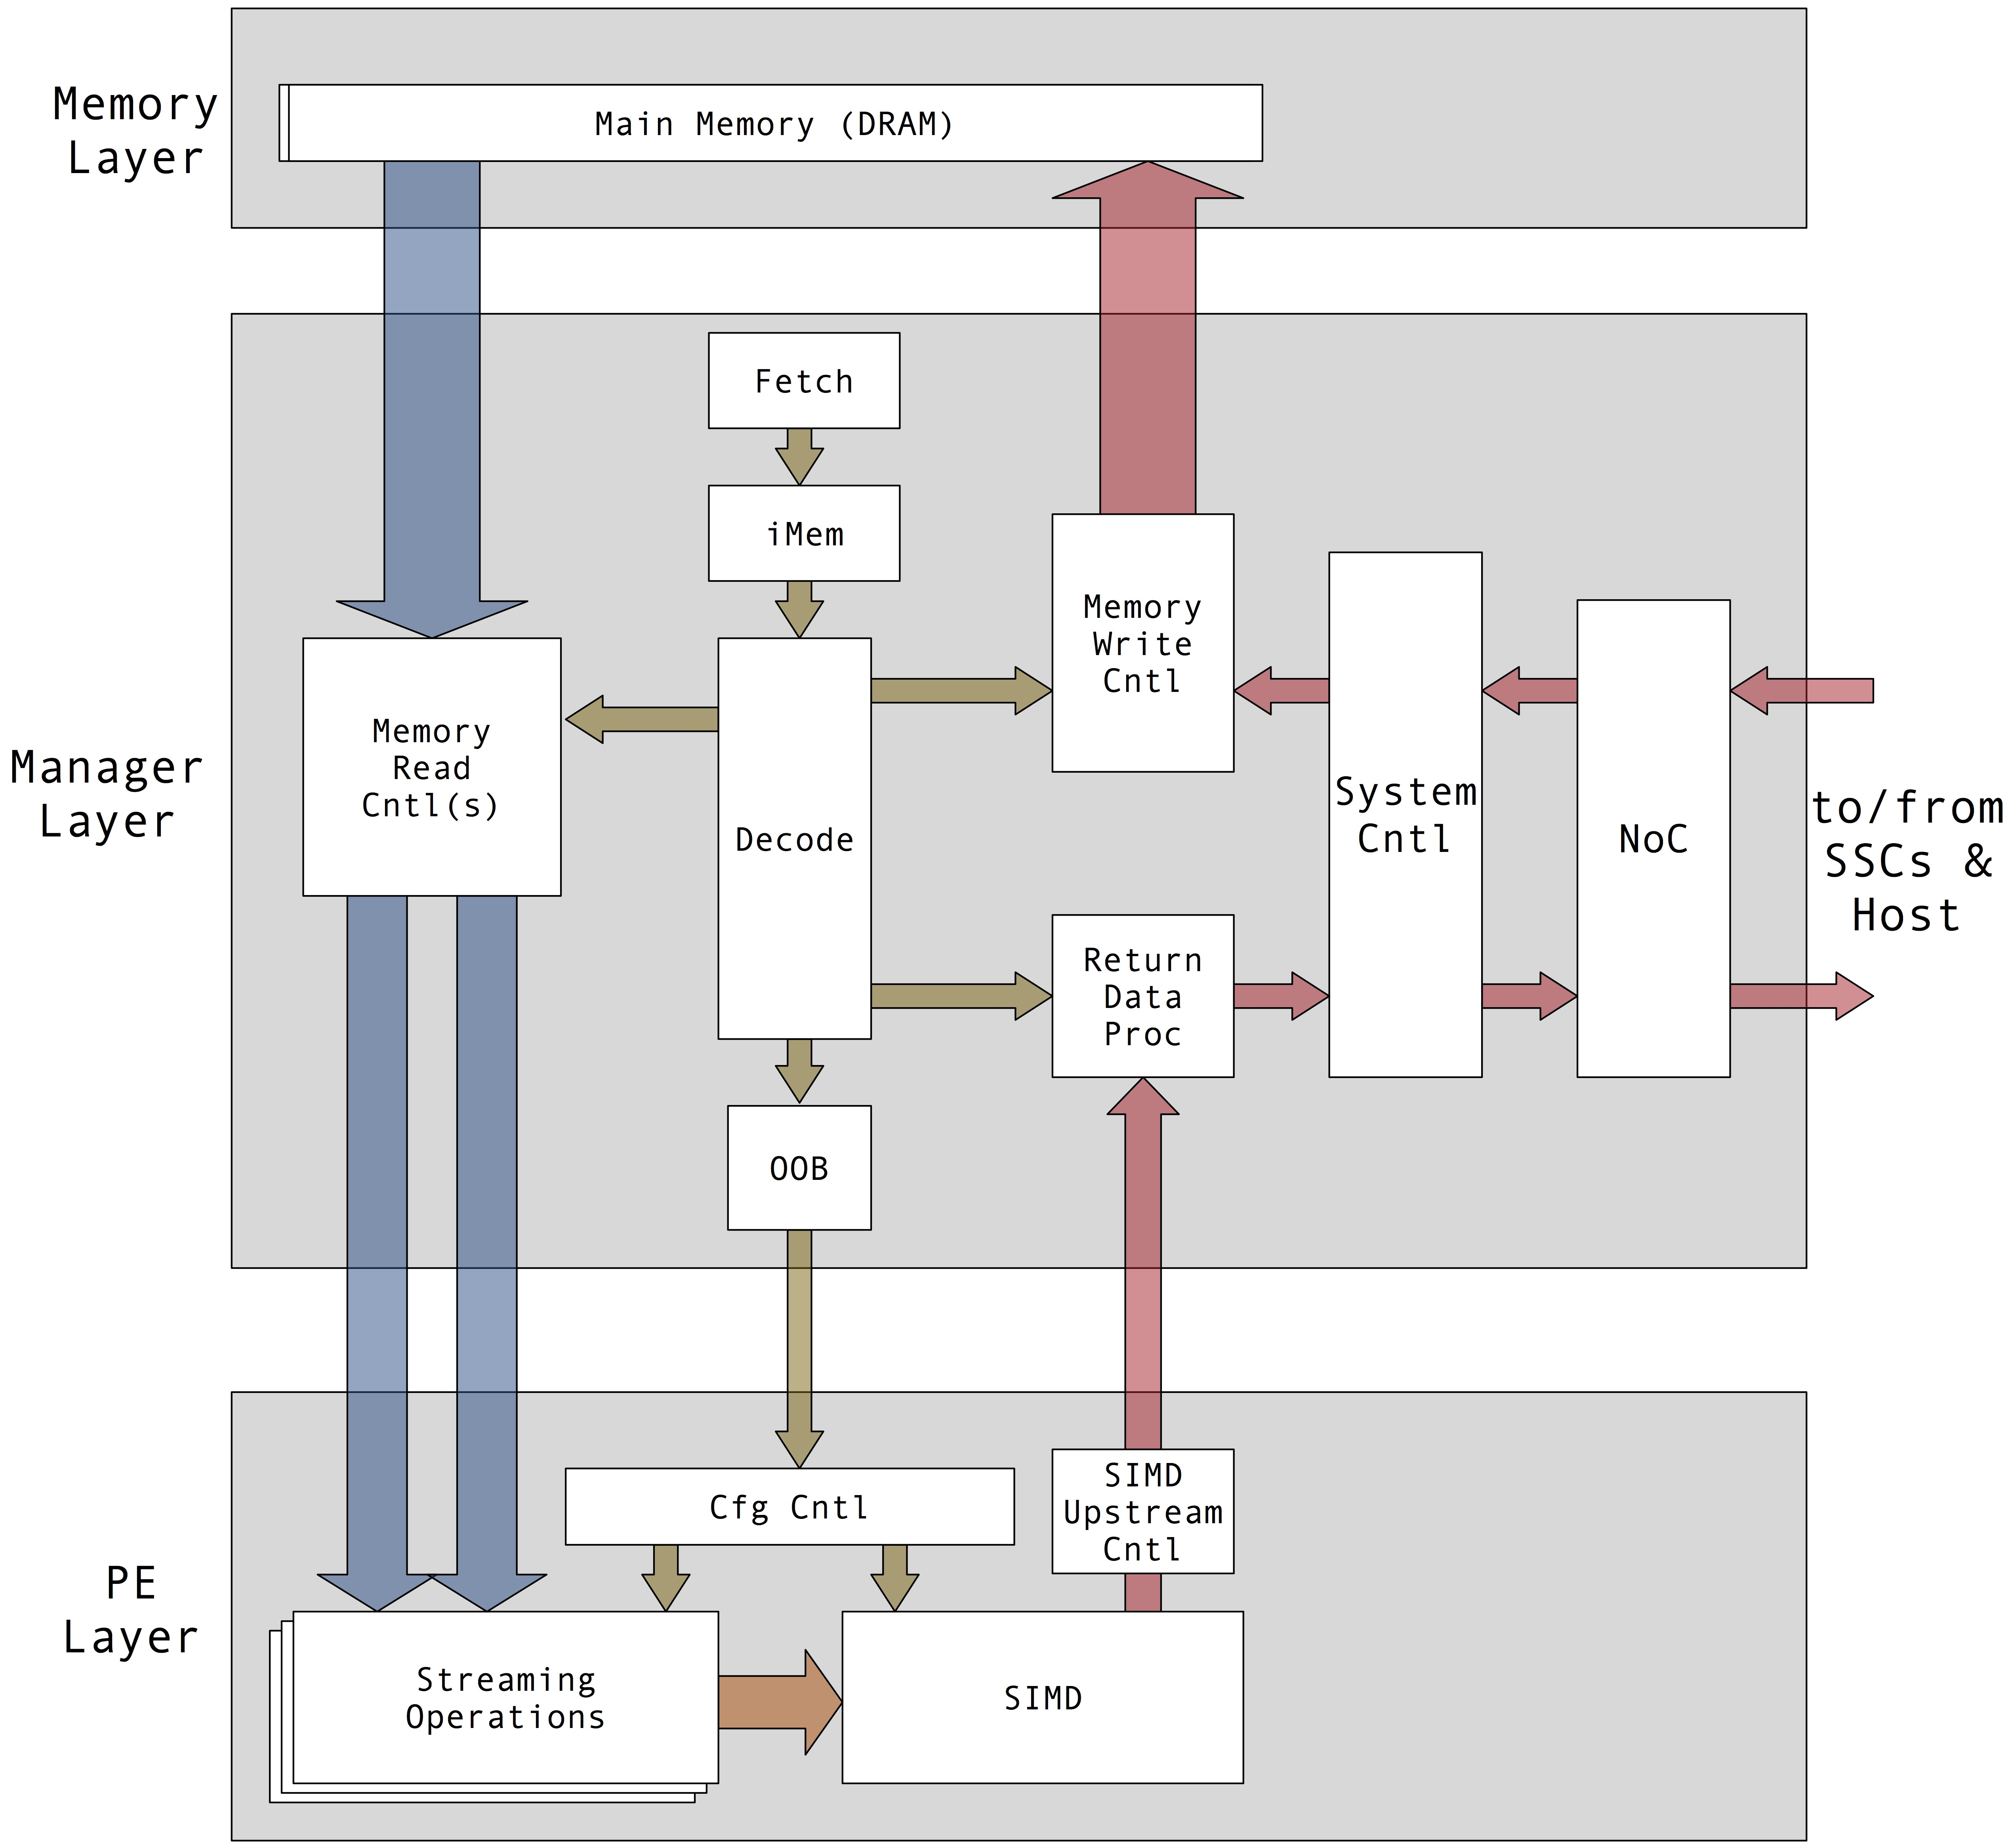
\includegraphics[width=2.75in]{DetailedFlowDiagram.jpg}}
}
\center\caption{Sub-System Column (SSC) Block Diagram}
\label{fig:DetailedFlowDiagram}
\end{figure}

\fi

\iffalse

\begin{figure*}[!t]
% the [] contains position info e.g. [!t] means here
\centering
\captionsetup{justification=centering}
\centerline{
\mbox{
\includegraphics[width=6.0in]{DetailedBlockDiagram.jpg}}
}
\center\caption{Sub-System Column (SSC) Detailed Block Diagram}
\label{fig:DetailedBlockDiagram}
\end{figure*}

\fi

\iffalse


\section{Detailed System Description}
\label{sec:detailedSystemDescription}

A detailed flow diagram and block diagram of the sub-system column can be seen in Figures \ref{fig:DetailedFlowDiagram} and \ref{fig:DetailedBlockDiagram} respectively.
\begin{figure}[!t]
% the [] contains position info e.g. [!t] means here
\centering
\captionsetup{justification=centering}
\captionsetup{width=.9\linewidth}
\centerline{
\mbox{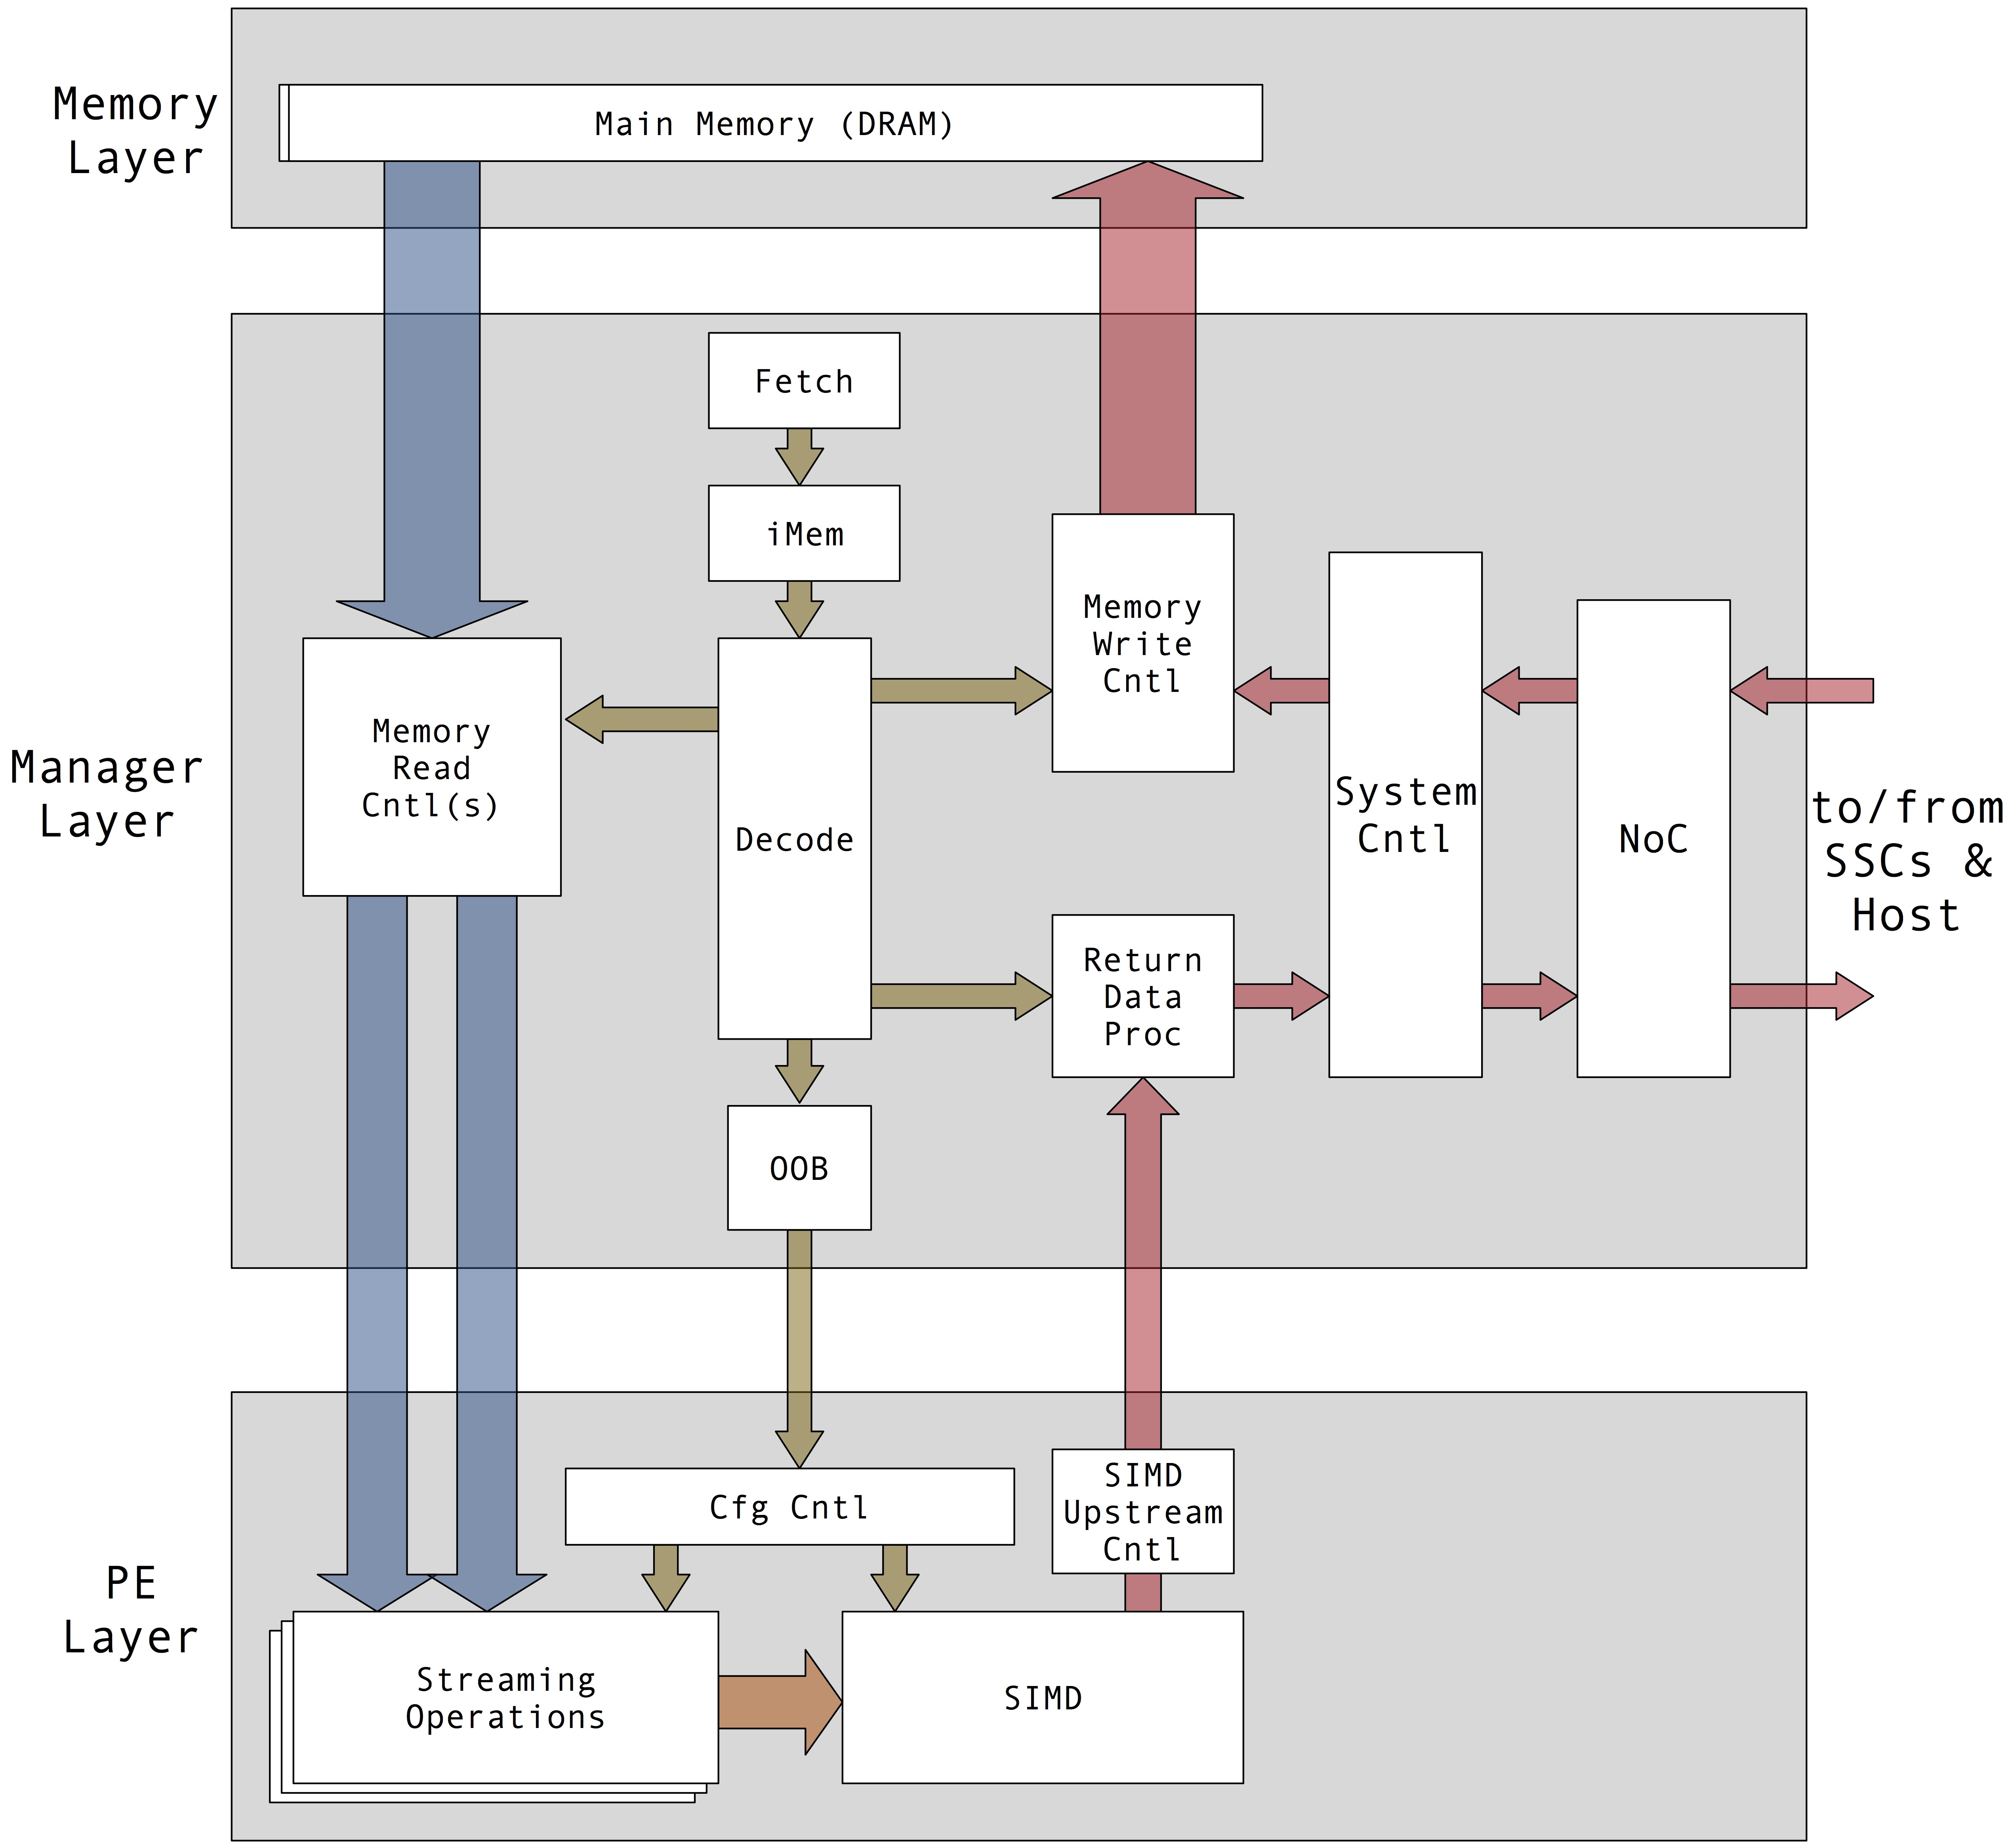
\includegraphics[width=2.75in]{DetailedFlowDiagram.jpg}}
}
\center\caption{Sub-System Column (SSC) Detailed Flow Diagram}
\label{fig:DetailedFlowDiagram}
\end{figure}

\begin{figure*}[!t]
% the [] contains position info e.g. [!t] means here
\centering
\captionsetup{justification=centering}
\centerline{
\mbox{
\includegraphics[width=6.0in]{DetailedBlockDiagram.jpg}}
}
\center\caption{Sub-System Column (SSC) Detailed Block Diagram}
\label{fig:DetailedBlockDiagram}
\end{figure*}

\subsection{Manager}
\label{sec:manager}

\subsubsection{Operation Decode}
\label{ssec:operationDecode}

In Figure \ref{fig:DetailedBlockDiagram}, instructions are read from instruction memory and passed to the instruction decoder.

The operation tuple is decoded and a streaming operation (stOp) pointer and a \ac{simd} operation pointer are sent to the PE inside an OOB control packet.

The stOp pointer specifies what streaming operation is to take place on the data directly streamed to the PE. In the baseline system, typically this would be a floating-point multiply accumulate on two arguments, the pre-synaptic neuron states and the pre-synaptic weights.

The \ac{simd} pointer is essentially a program counter that will be invoked when the stOp result is passed to the \ac{simd}.

Note that other types of stOp includes a NOP with a destination of local memory. This allows us to transfer block of instruction or data from the manager to the PE.


\subsubsection{Argument Decode}
\label{ssec:argumentDecode}
The instruction also includes argument descriptors. These descriptors include a storage descriptor pointers that point to a storage descriptor stored in local memory that encodes where data should be read from for the one or two arguments that will be streamed from \ac{dram} to the stOp within the PE. In the case of a \ac{an} activation calculation, there are two arguments, the pre-synaptic neuron states and the pre-synaptic weights. The read storage descriptor pointers are passed to the Memory Read Controllers (MRC). The MRCs read the actual storage descriptor from their local memory and immediately start sending read commands to the memory via a Main Memory Controller (MMC). The MMC is not shown in the diagram but essentially takes the memory read requests and converts them into the \ac{dram} read protocol.

As soon as read data is sent back to the MRC via the MMC, that data is aligned with to the 32 Streaming Operations inside the PE.


\subsubsection{Result data Processing}
\label{ssec:resultDataprocessing}
The instruction also includes argument descriptors. These descriptors include a storage descriptor pointers that point to a storage descriptor stored in local memory that encodes where data should be read from for the one or two arguments that will be streamed from \ac{dram} to the stOp within the PE. In the case of a \ac{an} activation calculation, there are two arguments, the pre-synaptic neuron states and the pre-synaptic weights. The read storage descriptor pointers are passed to the Memory Read Controllers (MRC). The MRCs read the actual storage descriptor from their local memory and immediately start sending read commands to the memory via a Main Memory Controller (MMC). The MMC is not shown in the diagram but essentially takes the memory read requests and converts them into the \ac{dram} read protocol.

As soon as read data is sent back to the MRC via the MMC, that data is aligned with the downstream bus and sent to the 32 Streaming Operations inside the PE.


\subsubsection{Memory Write Controller}
\label{ssec:memoryWriteController}

The Memory Write Controller (MWC) receives data from to sources, the NoC via the MCNTL and the RDP.

In both cases, the MWC read the actual storage descriptor from their local memory and immediately start forming data that will be written back to main memory.

When the data is formed, a write command is sent to the memory via the MMC. Again, the MMC is not shown in the diagram but takes the memory write requests along with the data and converts them into the \ac{dram} write protocol.

The MWC can only operate on one of the two sources at any one time. However, there are four 4096-bit holding registers where data is formed prior to the write request.

The holding registers have the potential in future to allow aggregation of data from one or more operations to allow a coalesced write back to main memory.


\subsection{Processing Engine}
\label{sec:pe}

\subsubsection{Configuration}
\label{ssec:peConfiguration}

A configuration controller within the PE (PE\_CNTL) takes the OOB packet from the Manager and extracts the stOp and \ac{simd} operation pointers.

The stOp pointer is used to point to a local stOp configuration memory. The memory contains the various configuration data required by the streaming operation controller (stOp\_CNTL). The stOp\_CNTL is not shown.

The stOp\_CNTL configures the:

\begin{outline}
    \1 Operation type
    \1 Number of active execution lanes
    \1 Source of the argument data, which can be downstream data from the manager or from the small local \ac{sram}
    \1 Destination of the result data, which can be the \ac{simd} or the small local \ac{sram}
\end{outline}

The \ac{simd} operation pointer is sent to the \ac{simd}.

\subsubsection{Streaming Operations}
\label{ssec:stOps}

The streaming Operations (stOp) are designed to operate on data passed from the Manager at or near line-rate. If line-rate c\ac{ann}ot be maintained, a flow-control mechanism is employed to slow the data from the Manager.

Once the stOp has processed the data, it passes the result to the \ac{simd}. Note in some cases the result can be placed in local \ac{sram} or sent to both \ac{simd} and \ac{sram}.

It should also be stated that while the stOp is processing the current data, the \ac{simd} may be operating on the result of the previous operation. It is expected the \ac{simd} will have completed the previous operation before the stOp completes the current operation, but again, if necessary a flow control mechanism between \ac{simd} and stOP will be engaged if the \ac{simd} is not ready.

\subsubsection{SIMD}
\label{ssec:simd}

The \ac{simd} takes the result data and performs the operation starting at the program counter (PC) indicated by the \ac{simd} operation pointer provided by the PE\_CNTL.

The stOp provides the result to the \ac{simd} via a local register. The result is also written, in most cases to the small local \ac{sram}.

The \ac{simd} performs the specified operation on the data provided by the stOp.

In most cases this will be the \ac{an} activation function and in the baseline system is the Rectified Linear function (ReLu).

When the \ac{simd} has completed its operation, it passes the result to the \ac{simd} Upstream controller to be returned to the Manager.

\subsubsection{Result Data}
\label{ssec:result}

The \ac{simd} Upstream Controller (SUI) takes the data and encapsulates it in an Upstream packet. Included in the packet is the tag required by the Return Data processor within the Manager.

\fi


% #######################################################################################################################################
% >>>>>>>>>>>>>>>>>>>>>>>>>>> Results <<<<<<<<<<<<<<<<<<<<<<
\section{Results}
\label{sec:Results}
The objective of this work was to design a system able to accelerate multiple disparate \acp{ann} in embedded systems.
Given that these systems cannot effectively utilize \ac{sram}, the main objective was to demonstrate a system that can operate efficiently using a customized \ac{3ddram} with a very wide data-bus.
\ac{3dic} technology was exploited, including \ac{3ddram}, because a major theme of this work is that \ac{3dic} provides many benefits, including reduced energy use, lower area requirements, and high bandwidth. 
It was necessary to show that the proposed system can maintain the required data bandwidth while staying within the physical footprint of the \ac{3ddram}. 

Because its the technology node employed for some recent \acp{gpu} and other \acp{asic} such as \cite{jouppi2017datacenter}, the target technology chosen was 28nm.
The 28nm standard cell library available to this team did not have register files, therefore the design was synthesized using an available 65nm technology node and then scaled to 28nm.
Some representative portions of the design were synthesized using the \SI{28}{\nano\meter} libraries to obtain scaling numbers.
The final scaling numbers are shown in Table \ref{tab:Scaling numbers}.

\begin{figure*}[!htbp]
  % the [] contains position info e.g. [!t] means here
  \centering
  \captionsetup{justification=centering}
    \begin{minipage}{0.85\textwidth}
        \vspace{5mm}
        \begin{adjustbox}{width=1\textwidth}
            \footnotesize
            \begin{tabular}{|>{\centering}m{1cm}|>{\centering}m{1cm}|>{\centering}m{1cm}|>{\centering}m{1.3cm}|>{\centering}m{1.3cm}|>{\centering}m{1cm}|>{\centering}m{1.3cm}|m{1.3cm}|}\cline{3-8}
              %\hline
              %\rowcolor{gray!50}
              %\multicolumn{5}{|c|}{Power } \\
              %\hline
              %\rowcolor{gray!25}  
         \multicolumn{2}{c|}{}                                          & \multicolumn{3}{c|}{Logic power}                                                                  &  \multicolumn{3}{c|}{Memory power}                                                                                                                                  \\\cline{1-8}
         Logic Area                  & Memory Area                      & Internal                            & Net switching                  & Leakage                    & Internal                                                                                                              & Net switching                  & Leakage    \\\cline{1-8}
          \num{2.68}                 & \num{2.78}                       &  \num{5.07}                         & \num{1.21}                     & \num{4.12e-4}              &  \num{5.07}  & NA                             & NA         \\
              \hline
            \end{tabular}
        \end{adjustbox}
      %\subcaption{Example design area}
      %\label{tab:Example design area}
  \end{minipage}
  \captionsetup{justification=centering, skip=9pt}
  \vspace{0.0cm}
  \captionof{table}{\SI{68}{\nano\meter} to \SI{28}{\nano\meter} scaling numbers}
  \label{tab:Scaling numbers}
\end{figure*}

The primary control and datapaths of the system have been simulated in a system verilog environment. 
\iffalse
It has been synthesized using a 65nm technology node.
\fi
%The design has been coded . 
Initial synthesis timing closure at a frequency of \SI{500}{\mega\hertz} is complete.
Initial place and route for the Manager and PE are shown in Figure \ref{fig:Manager and PE Die layouts}. 
The area contribution of each block within the Manager and PE can be seen in Table \ref{tab:Area contribution}.
\begin{table}[h]
%  \captionsetup{justification=centering, skip=-5pt}
  \captionsetup{justification=centering, skip=3pt}
  \caption{Area Contribution}
  \vspace{3pt}
  \label{tab:Area contribution}
  \centering
    % [lr] ~ left align col 0 and right align col 1
    % e.g. 4 columns could be lccr
  \begin{subtable}{0.5\textwidth}
    \centering
    \begin{adjustbox}{width=0.75\textwidth}
      \begin{tabular}{ccc}
        \toprule
                            % \multicolumn{4}{c}{3D-\ac{dram} Simulation-based estimates}   \\
                         &          &                                         \\  %\cline{1-1}
            Block        &Instances &Percentage                               \\  %\cline{1-1}
            Name         &          &Contribution                             \\  %\cline{1-1}
        \hline  % instead of \midrule %midrule doesnt overlap with column lines
  Memory Controller      & 1&\SI[per-mode=symbol]{15.0}{\percent}  \\ 
        NoC              & 1&\SI[per-mode=symbol]{ 7.1}{\percent}  \\
        Read Control     & 2&\SI[per-mode=symbol]{53.1}{\percent}  \\
        Write Control    & 1&\SI[per-mode=symbol]{ 7.4}{\percent}  \\
      Instruction Proc   & 1&\SI[per-mode=symbol]{ 1.6}{\percent}  \\
      Return Data Proc   & 1&\SI[per-mode=symbol]{ 1.6}{\percent}  \\
        Misc             & 1&\SI[per-mode=symbol]{14.2}{\percent}  \\
        \bottomrule
      \end{tabular}
    \end{adjustbox}
    \vspace{3pt}
    \captionsetup{justification=centering, skip=10pt}
    \caption{Manager}
    \label{tab:Manager Area Contribution}
  \end{subtable}
  \bigskip
  \begin{subtable}{0.5\textwidth}
    \centering
    \begin{adjustbox}{width=0.85\textwidth}
      \begin{tabular}{ccc}
        \toprule
                            % \multicolumn{4}{c}{3D-\ac{dram} Simulation-based estimates}   \\
                         &          &                                          \\  %\cline{1-1}
            Block        &Instances & Percentage                               \\  %\cline{1-1}
            Name         &          & Contribution                             \\  %\cline{1-1}
        \hline  % instead of \midrule %midrule doesnt overlap with column lines
     Operation Decode    & 1&\SI[per-mode=symbol]{ 3.4}{\percent}  \\
   Return Data Control   & 1&\SI[per-mode=symbol]{ 1.5}{\percent}  \\
    SIMD Control         & 1&\SI[per-mode=symbol]{ 8.1}{\percent}  \\
        SIMD             & 1&\SI[per-mode=symbol]{19.3}{\percent}  \\
  Streaming Operations   &32&\SI[per-mode=symbol]{43.3}{\percent}  \\
  Streaming Op Control   & 1&\SI[per-mode=symbol]{ 2.1}{\percent}  \\
 Local Memory + Control\footnote{A small amount of scratchpad memory was provided between stOps and \ac{simd} but in practice could be much smaller. It is not used in any of the fanin tests.}  & 1&\SI[per-mode=symbol]{17.7}{\percent}  \\ 
        Misc             & 1&\SI[per-mode=symbol]{ 4.6}{\percent}  \\
        \bottomrule
      \end{tabular}
    \end{adjustbox}
    \vspace{3pt}
    \captionsetup{justification=centering, skip=10pt}
    \caption{PE}
    \label{tab:PE Area Contribution}
  \end{subtable}
  \end{table}

The parasitics were extracted from these layouts and simulated against a group of operations. 
The operations simulated were based on the expected lower and upper limits of pre-synaptic fanin. 
These testcases were based on layers similar to CONV2 and FC-7 from \cite{krizhevsky2012imagenet} and represent a pre-synaptic fanin of 225 and 4000 respectively.
Additional testcases were employed representing pre-synaptic fanins of 294, 300, 500 and 1000. Both locally connected (CONV) and fully connected (FC) type fanins were tested.
The results showing sustained average bandwidth can be seen in Table \ref{tab:Bandwidth Estimates}.

The simulation generated an activity file which was then used by the Synopsys\textregistered ~Primetime-PX\texttrademark ~power analysis tool to obtain power and bandwidth estimates.
The \ac{dram} accesses were captured and \ac{dram} energy dissipation calculated from \cite{tezzaron:diram4}. The power dissipated in the TSVs were estimated from \cite{liu2012compact}.
These estimates were used to estimate power dissipation for operating frequencies of \SI{500}{\mega\hertz} and \SI{700}{\mega\hertz}.
The estimated overall power along with per block contribution are shown in Table \ref{tab:Simulation-based estimates}.

\begin{table}[h]
%  \captionsetup{justification=centering, skip=-5pt}
  \captionsetup{justification=centering, skip=3pt}
  \caption{Power Estimates}
  \vspace{3pt}
  \label{tab:Simulation-based estimates}
  \centering
    % [lr] ~ left align col 0 and right align col 1
    % e.g. 4 columns could be lccr
  \begin{subtable}{0.5\textwidth}
    \centering
    \begin{adjustbox}{width=0.85\textwidth}
      \begin{tabular}{cccc}
        \toprule
                            % \multicolumn{4}{c}{3D-\ac{dram} Simulation-based estimates}   \\
                         &                       & Total    &                                          \\  %\cline{1-1}
            Technology   & Clock                 & Expected &                                          \\  %\cline{1-1}
                Node     & Frequency             &  Power   &  Testcase                                \\  %\cline{1-1}
        \hline  % instead of \midrule %midrule doesnt overlap with column lines
                   28nm  & \SI{500}{\mega\hertz} &   64W    &  CONV-294\iffalse \SI[per-mode=symbol]{\sim 70}{\percent} \fi \\ %\cline{2-2}
                   28nm  & \SI{700}{\mega\hertz} &   88W    &  CONV-294\iffalse \SI[per-mode=symbol]{\sim 70}{\percent} \fi \\ %\cline{2-2}
        \bottomrule
      \end{tabular}
    \end{adjustbox}
    \vspace{3pt}
    \captionsetup{justification=centering, skip=10pt}
    \caption{Power Dissipation}
    \label{tab:Power Dissipation}
  \end{subtable}
  \bigskip
  \begin{subtable}{0.5\textwidth}
    \centering
    \begin{adjustbox}{width=0.55\textwidth}
      \begin{tabular}{cc}
        \toprule
                            % \multicolumn{4}{c}{3D-\ac{dram} Simulation-based estimates}   \\
                         &                                          \\  %\cline{1-1}
            Block        & Percentage                               \\  %\cline{1-1}
            Name         & Contribution                             \\  %\cline{1-1}
        \hline  % instead of \midrule %midrule doesnt overlap with column lines
                Manager  & \SI[per-mode=symbol]{66.6}{\percent}  \\ 
                     PE  & \SI[per-mode=symbol]{28.0}{\percent}  \\
                   \ac{dram}  & \SI[per-mode=symbol]{ 2.5}{\percent}  \\
              \ac{dram} TSVs  & \SI[per-mode=symbol]{ 1.8}{\percent}  \\
         Stack Bus TSVs  & \SI[per-mode=symbol]{ 1.2}{\percent}  \\
        \bottomrule
      \end{tabular}
    \end{adjustbox}
    \vspace{3pt}
    \captionsetup{justification=centering, skip=10pt}
    \caption{Power Contribution}
    \label{tab:Power Dissipation}
  \end{subtable}
  \end{table}

As bus efficiency is the main metric, Table \ref{tab:Bandwidth Estimates} shows sustained average bandwidth over the fanin testcases.

\begin{table}[h]
%  \captionsetup{justification=centering, skip=-5pt}
  \captionsetup{justification=centering, skip=3pt}
  \caption{Fanin Bandwidth Tests}
  \vspace{3pt}
  \label{tab:Bandwidth Estimates}
  \centering
    \begin{adjustbox}{width=0.37\textwidth}
      \begin{tabular}{ccc}
        \toprule
                            % \multicolumn{4}{c}{3D-\ac{dram} Simulation-based estimates}   \\
                                                       &                                         \multicolumn{2}{c}{Average Bandwidth}                      \\  %\cline{1-1}
                                                       &                                         \multicolumn{2}{c}{At Frequency}                                      \\  %\cline{1-1}
                   Test                                &        \SI{500}{\mega\hertz}                            & \SI{700}{\mega\hertz}                               \\  %\cline{1-1}
        \hline  % instead of \midrule %midrule doesnt ove        
                   CONV2 \cite{krizhevsky2012imagenet} &\ \SI[per-mode=symbol]{\sim 25}{\tera\bit\per\second}    & \SI[per-mode=symbol]{\sim 35}{\tera\bit\per\second} \\ %\cline{2-2}
                   CONV-294                            &\ \SI[per-mode=symbol]{\sim 26}{\tera\bit\per\second}    & \SI[per-mode=symbol]{\sim 37}{\tera\bit\per\second} \\ %\cline{2-2}
                   CONV-300                            &\ \SI[per-mode=symbol]{\sim 27}{\tera\bit\per\second}    & \SI[per-mode=symbol]{\sim 37}{\tera\bit\per\second} \\ %\cline{2-2}
                   CONV-500                            &\ \SI[per-mode=symbol]{\sim 29}{\tera\bit\per\second}    & \SI[per-mode=symbol]{\sim 41}{\tera\bit\per\second} \\ %\cline{2-2}
                   CONV-1000                           &\ \SI[per-mode=symbol]{\sim 31}{\tera\bit\per\second}    & \SI[per-mode=symbol]{\sim 43}{\tera\bit\per\second} \\ %\cline{2-2}
                   CONV-2500                           &\ \SI[per-mode=symbol]{\sim 32}{\tera\bit\per\second}    & \SI[per-mode=symbol]{\sim 45}{\tera\bit\per\second} \\ %\cline{2-2}
                   FC-350                              &\ \SI[per-mode=symbol]{\sim 28}{\tera\bit\per\second}    & \SI[per-mode=symbol]{\sim 39}{\tera\bit\per\second} \\ %\cline{2-2}
                   FC-500                              &\ \SI[per-mode=symbol]{\sim 29}{\tera\bit\per\second}    & \SI[per-mode=symbol]{\sim 41}{\tera\bit\per\second} \\ %\cline{2-2}
                   FC-1000                             &\ \SI[per-mode=symbol]{\sim 31}{\tera\bit\per\second}    & \SI[per-mode=symbol]{\sim 43}{\tera\bit\per\second} \\ %\cline{2-2}
                   FC-7 \cite{krizhevsky2012imagenet}  &\ \SI[per-mode=symbol]{\sim 32}{\tera\bit\per\second}    & \SI[per-mode=symbol]{\sim 45}{\tera\bit\per\second} \\ %\cline{2-2}
        \bottomrule
      \end{tabular}
    \end{adjustbox}
    \vspace{3pt}
  \end{table}

%%%%\begin{table}[h]
%%%%%  \captionsetup{justification=centering, skip=-5pt}
%%%%  \captionsetup{justification=centering, skip=3pt}
%%%%  \caption{Design targets}
%%%%  \label{tab:DesignTargets}
%%%%  \centering
%%%%%  \begin{center}
%%%%    % [lr] ~ left align col 0 and right align col 1
%%%%    % e.g. 4 columns could be lccr
%%%%    \begin{tabular}{lccccc}
%%%%          \toprule
%%%%                            %& \multicolumn{4}{c}{Technology}   \\
%%%%                            &       &       &  Usable    &          &  \\  %\cline{1-1}
%%%%                            &       &       &   \ac{dram}     & Expected &  \\  %\cline{1-1}
%%%%                            & Tech  & Freq  & Bandwidth  &  Power   &  \\  %\cline{1-1}
%%%%          \hline  % instead of \midrule %midrule doesnt overlap with column lines
%%%%                  3D-System & 28    & \SI{700}{\mega\hertz}      &       \SI[per-mode=symbol]{\sim 64}{\tera\bit\per\second}   &  73W   &  \\ %\cline{2-2}
%%%%                  NVidia    & 28    &       &  $\ll$\SI[per-mode=symbol]{1.28}{\tera\bit\per\second} &  100W  &  \\
%%%%                  TPU       & 28    &       &  $<$  \SI[per-mode=symbol]{224}{\giga\bit\per\second}  &  40W   &  \\
%%%%          \bottomrule
%%%%    \end{tabular}
%%%%%  \end{center}
%%%%\end{table}



\begin{figure}
\centering
\begin{subfigure}{.25\textwidth}
  \centering
  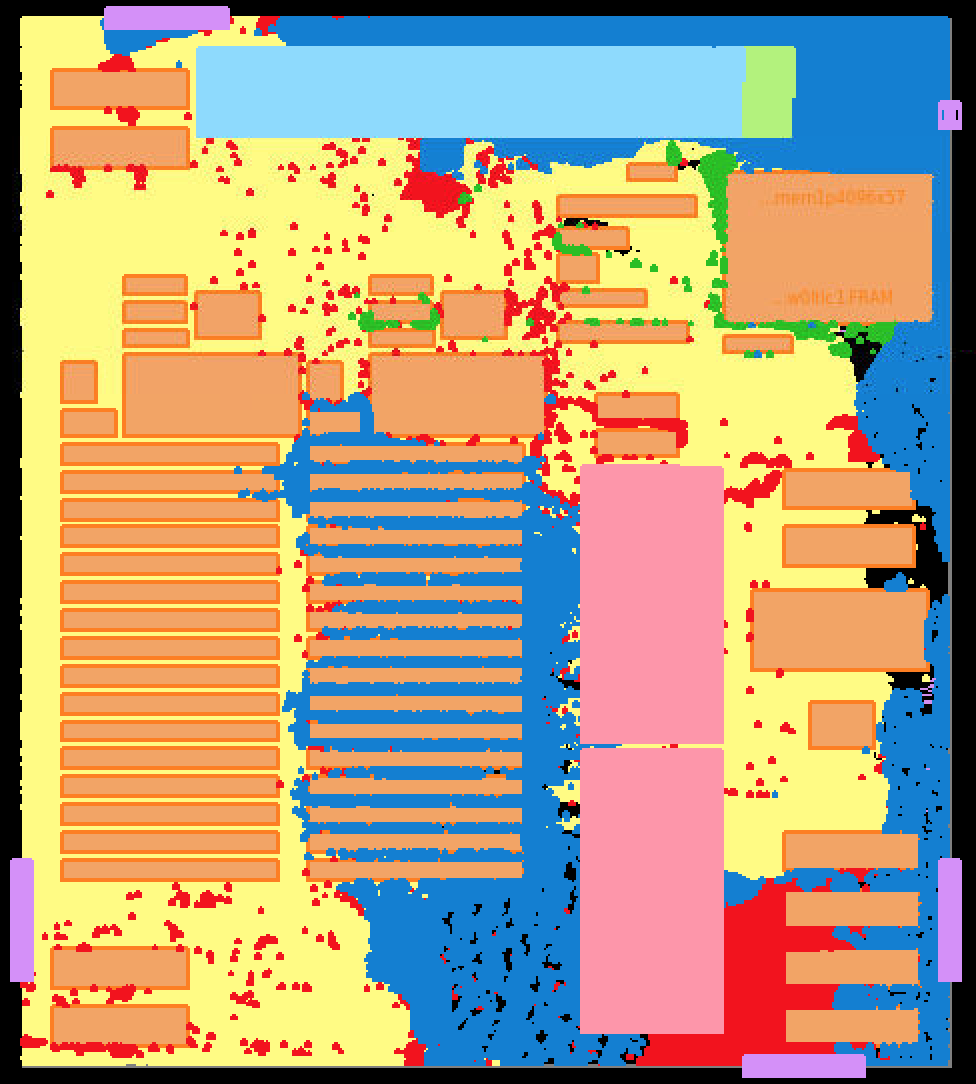
\includegraphics[width=0.95\textwidth]{ManagerLayout.png}
  \captionsetup{justification=centering, width=.8\linewidth}
  \caption{Manager}
  \label{fig:managerLayout}
\end{subfigure}%
\begin{subfigure}{.25\textwidth}
  \centering
  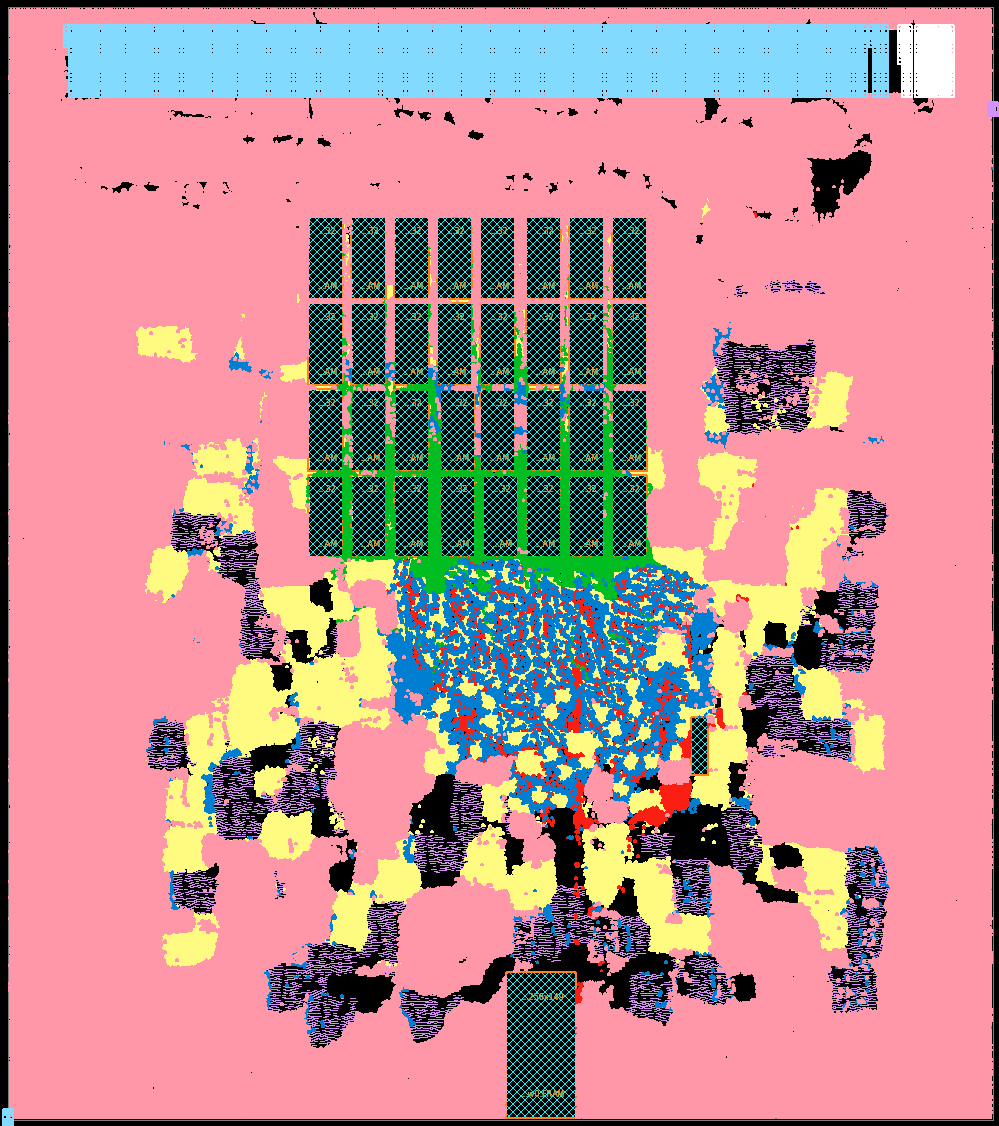
\includegraphics[width=0.95\textwidth]{PElayout.png}
  \captionsetup{justification=centering, width=.8\linewidth}
  \caption{PE}
  \label{fig:peLayout}
\end{subfigure}
\captionsetup{justification=centering, width=.9\linewidth}
\caption{Manager and PE Die layouts}
\label{fig:Manager and PE Die layouts}
\end{figure}


%%%%\begin{figure}[h]
%%%%\centering
%%%%\captionsetup{justification=centering}
%%%%    \begin{subtable}{.50\textwidth}
%%%%    %  \captionsetup{justification=centering, skip=-5pt}
%%%%      \centering
%%%%    %  \begin{center}
%%%%        % [lr] ~ left align col 0 and right align col 1
%%%%        % e.g. 4 columns could be lccr
%%%%        \resizebox{\textwidth}{!}{ % Scale table
%%%%        \begin{tabular}{r|ccc}
%%%%          \toprule
%%%%                         & \multicolumn{3}{c}{Technology} \\
%%%%                    Unit & \SI{130}{\nm} & \SI{65}{\nm} & \SI{45}{\nm}  \\
%%%%          \hline
%%%%          SIMD (32-lane) & 3200000 \\
%%%%                    DMA  &               & 368000  \\
%%%%      Memory Controller  &               & 294000  \\
%%%%                Control  &               & 1032000 \\
%%%%                   \ac{sram}  &               & 740098  \\
%%%%                    FMA  &               &              & 405440 \\
%%%%          \bottomrule
%%%%        \end{tabular}
%%%%        }
%%%%      \captionsetup{justification=centering, skip=9pt}
%%%%      \vspace{-1mm}
%%%%      \caption{Original area estimates}
%%%%      \label{tab:areaEstimates}
%%%%    %  \end{center}
%%%%    \end{subtable}
%%%%    \hfill
%%%%    %\vfill
%%%%    \begin{subtable}{.45\textwidth}
%%%%    %  \captionsetup{justification=centering, skip=-5pt}
%%%%      \centering
%%%%    %  \begin{center}
%%%%        % [lr] ~ left align col 0 and right align col 1
%%%%        % e.g. 4 columns could be lccr
%%%%        \resizebox{\textwidth}{!}{%
%%%%        \begin{tabular}{r|cccc}
%%%%          \toprule
%%%%                            %& \multicolumn{4}{c}{Technology}   \\
%%%%                            &       &  Usable    &          &  \\  %\cline{1-1}
%%%%                            &       &   \ac{dram}     & Expected &  \\  %\cline{1-1}
%%%%                            & Tech  & Bandwidth  &  Power   &  \\  %\cline{1-1}
%%%%          \hline  % instead of \midrule %midrule doesnt overlap with column lines
%%%%                  3D-System & 28    &       \SI[per-mode=symbol]{\sim 64}{\tera\bit\per\second}   &  73W   &  \\ %\cline{2-2}
%%%%                  NVidia    & 28    &  $\ll$\SI[per-mode=symbol]{1.28}{\tera\bit\per\second} &  100W  &  \\
%%%%                  TPU       & 28    &  $<$  \SI[per-mode=symbol]{224}{\giga\bit\per\second}  &  40W   &  \\
%%%%          \bottomrule
%%%%        \end{tabular}
%%%%        }
%%%%      \captionsetup{justification=centering, skip=9pt}
%%%%      \vspace{3mm}
%%%%      \caption{Scaling numbers (from \cite{schabel2014energy})}
%%%%      \label{tab:scalingNumbers}
%%%%    %  \end{center}
%%%%    \end{subtable}
%%%%\vspace{-2mm}
%%%%\caption{Original area estimates and scaling numbers}
%%%%\label{fig:areaAndScalingEstimates}
%%%%\end{figure}


% #######################################################################################################################################
% >>>>>>>>>>>>>>>>>>>>>>>>>>> Conclusions and Further Work <<<<<<<<<<<<<<<<<<<<<<
\section{Conclusions}
\label{sec:Conclusions}
There have been many attempts to accelerate \acp{ann}. Many have shown excellent performance mainly when implementing \acp{cnn}. The improvement mostly comes from the ability to 
hold kernel weights and/or \ac{an} activations in local \ac{sram}. Another method of employing local memory is often due to pooling of batch requests, especially in server applications.
This local storage allows the system to take advantage of the low latency and random access benefits of \ac{sram} whilst performing multiple operations on that data.
When considering applications where this local storage cannot be used effectively, all these implementations suffer a large degradation in performance.

This work considers embedded applications where a system is processing requests with a disparate set of \acp{ann}. The assumption is that local \ac{sram} is no longer effective and performance is based on \ac{dram} bandwidth.
This work considers 3DIC technology and a customized 3D-\ac{dram} is proposed. 

The customized 3D-\ac{dram} combined with a design based on custom instructions and operation descriptors allows the system to achieve high levels of memory bandwidth efficiency.

There is no doubt existing \ac{cnn} accelerators that take advantage of batch processing achieve a performance that is difficult to better, but applying these systems to this works target application exposes those systems \ac{dram} bandwidth limitations.
This work demonstrates a \ac{3dic} system that at the surface provides relatively low \ac{flops}, but considering the target application is memory bound, this work demonstrates a 3X power improvement and 6X area improvement over similar \ac{ann} systems \cite{chen2016diannao,azarkhish2017neurostream,kim2016neurocube,gao2017tetris}.

\section{Acknowlembeddedments}
\label{sec:Acknowlembeddedments}
This work was funded in part by DARPA and AFRL under FA8650-15-1-7518 and DARPA and ONR under N00014-17-1-3013, as part of the CHIPS program.

\iffalse
\section{Further Work}
\label{sec:Further Work}
This work does not put a high level of importance to the processing engine. The choice of using single-precision floating point format was in some part convenient. In fact, half-precision might have been a better choice especially as there
is a level of acceptance that lower precision is acceptable in \ac{ann} inference.
Therefore, further work should include :
\begin {outline}
  \1 Manager changes to support half-precision format
    \2 supports 16-bit FP would require additional muxing logic when directing words in the wide \ac{dram} bus to execution lanes, but the bulk of the design should remain relatively intact.
  \1 Half-Precision PE
    \2 modifying the PE to support 16-bit FP would be relatively trivial
  \1 Additional PE pipelining
    \2 Adding layers of processing to the PE would effectively increase the operations per second
      \3 the PE area utilization is relatively low so it could support some additional pipelining
      \3 using a reduction array would effectively double the FLOPs
      \3 looking at storing weights and inputs for a pipelined PE would be required and the manager would likely be customized to the PE, but the belief is the Manager design and complexity should be similar
  \1 Systolic PE
    \2 systolic arrays have shown efficacy when used in server applications such as TPU, but its not clear how effective they would be in an embedded application
      \3 consider how to effectively feed a systolic array PE
      \3 consider types of systolic array
      \3 consider situations such as multiple Managers feeding a single PE. For example, a systolic PE might use two managers to feed X and Y inputs of the array
 
\end{outline}
\fi


% Can use something like this to put references on a page
% by themselves when using endfloat and the captionsoff option.
\ifCLASSOPTIONcaptionsoff
  \newpage
\fi



% trigger a \newpage just before the given reference
% number - used to balance the columns on the last page
% adjust value as needed - may need to be readjusted if
% the document is modified later
%\IEEEtriggeratref{8}
% The "triggered" command can be changed if desired:
%\IEEEtriggercmd{\enlargethispage{-5in}}

% references section

% can use a bibliography generated by BibTeX as a .bbl file
% BibTeX documentation can be easily obtained at:
% http://mirror.ctan.org/biblio/bibtex/contrib/doc/
% The IEEEtran BibTeX style support page is at:
% http://www.michaelshell.org/tex/ieeetran/bibtex/
%\bibliographystyle{IEEEtran}
% argument is your BibTeX string definitions and bibliography database(s)
%
% <OR> manually copy in the resultant .bbl file
% set second argument of \begin to the number of references
% (used to reserve space for the reference number labels box)
%\nocite{*}
\bibliographystyle{IEEEtran}
\bibliography{IEEEabrv,IEEE_micro}
%\bibliography{Robot}
%\begin{thebibliography}{1}
%\bibitem{IEEEhowto:kopka}
%H.~Kopka and P.~W. Daly, \emph{A Guide to \LaTeX}, 3rd~ed.\hskip 1em plus
%  0.5em minus 0.4em\relax Harlow, England: Addison-Wesley, 1999.
%\end{thebibliography}

% biography section
% 
% If you have an EPS/PDF photo (graphicx package needed) extra braces are
% needed around the contents of the optional argument to biography to prevent
% the LaTeX parser from getting confused when it sees the complicated
% \includegraphics command within an optional argument. (You could create
% your own custom macro containing the \includegraphics command to make things
% simpler here.)
%\begin{IEEEbiography}[{\includegraphics[width=1in,height=1.25in,clip,keepaspectratio]{mshell}}]{Michael Shell}
% or if you just want to reserve a space for a photo:
\begin{IEEEbiographynophoto}{Lee B. Baker}
received a B.S. degree in Electrical Engineering from Brighton Polytechnic, UK, an M.S. degree in Electrical Engineering from Villanova University, USA and an M.B.A. degree from North Carolina State University, USA in 1983, 1994 and 2009 respectively. He earned his Ph.D. in Electrical and Computer Engineering from North Carolina State University in 2018.
His current research interests include acceleration of artificial neural networks.
\end{IEEEbiographynophoto}
% if you will not have a photo at all:
\begin{IEEEbiographynophoto}{Paul Franzon}
is currently the Cirrus Logic Distinguished Professor of Electrical and Computer Engineering at North Carolina State University.  He earned his Ph.D. from the University of Adelaide, Adelaide, Australia in 1988.  He has also worked at AT\&T Bell Laboratories, DSTO Australia, Australia Telecom and three companies he cofounded, Communica, LightSpin Technologies and Polymer Braille Inc. His current interests center on the technology and design of complex microsystems incorporating VLSI, MEMS, advanced packaging and nano-electronics. He has lead several major efforts and published over 300 papers in these areas.  In 1993 he received an NSF Young Investigators Award, in 2001 was selected to join the NCSU Academy of Outstanding Teachers, in 2003, selected as a Distinguished Alumni Professor, and received the Alcoa Research Award in 2005.  He served with the Australian Army Reserve for 13 years as an Infantry Solider and Officer.  He is a Fellow of the IEEE.
\end{IEEEbiographynophoto}

% You can push biographies down or up by placing
% a \vfill before or after them. The appropriate
% use of \vfill depends on what kind of text is
% on the last page and whether or not the columns
% are being equalized.

%\vfill

% Can be used to pull up biographies so that the bottom of the last one
% is flush with the other column.
%\enlargethispage{-5in}



% that's all folks
\end{document}


